\chapter{Neural network theory}
\label{chap:neural_network_theory}
Before tackling the local minimum problem, we must first understand the motivation and function of neural networks.
We will begin by introducing the general concept of supervised learning algorithms which neural networks are an example of.
This lays the foundation for a more rigorous definition of artificial neural networks in \ref{sec:ann} as regression models which we widen in the following section to include binary classification tasks as well.
The definitions, examples, and lemmata from this chapter are the groundwork for the stripe problem later on.

\section{Supervised learning}
At its core, the purpose of a neural network is to infer a function that maps some input to some output, based on sample input-output pairs.
In machine learning, we call this a \textit{supervised learning} task. 
Let us define that more precisely below.

\begin{definition}[Regression model]
    \label{def:reg_model}
    In machine learning, a regression model $R$ is defined as a mathematical function of the form $R:\mathbb{R}^D\rightarrow \mathbb{R}$ given by
    \begin{equation}
        \label{eq:reg_model}
        R(\vec{x}) = \hat{y} = y + \epsilon
    \end{equation}
    that models the relationship between a $D$-dimensional feature vector $\vec{x} \in \mathbb{R}^D$ of independent (\textit{input}) variables and the dependent (\textit{output}) variable $y \in \mathbb{R}$. 
    Given a particular $\vec{x}$, the model will produce a \textit{prediction} for $y$ which we denote $\hat{y}$.
    Here, the additive error term $\epsilon$ represents the discrepancy between $y$ and $\hat{y}$.
\end{definition}

\begin{definition}[Input space]
    \label{def:input_space}
    The input space $\mathcal{I}_R$ of a regression model $R$ is the set of all possible assignments to the feature vector $\vec{x}$.
    For a feature vector of $D$ dimensions,
    \begin{equation}
        \mathcal{I}_A=\mathbb{R}^D.
    \end{equation}
\end{definition}

\begin{definition}[Labelled dataset]
    \label{def:labelled_dataset}
    A labelled dataset consists of $N$ tuples of the form $\langle \vec{x}_i, y_i\rangle$ for $i=1,\dots,N$.
    For each feature vector $\vec{x}_i$ (a row vector), the corresponding $y_i$ represents the observed output, or \textit{label} \cite{burkov2019}.
    We use the vector
    \begin{equation}
        \label{eq:sup_learn_target}
        \vec{y} = \begin{bmatrix}
            y_1 & y_2 & \cdots & y_N
        \end{bmatrix}\tran
    \end{equation}
    to denote all the labelled outputs in the dataset, and the $N \times D$ matrix
    \begin{equation}
        \label{eq:sup_learn_input_matrix}
        \vec{X} = \begin{bmatrix}
            \vec{x}_1 & \vec{x}_2 & \cdots & \vec{x}_N
        \end{bmatrix}\tran
    \end{equation}
    for representing the corresponding feature vectors.
\end{definition}

\begin{definition}[Supervised learning]
    \label{def:supervised_learning}
    A supervised learning algorithm for a regression task infers the function $R$ given in \ref{eq:reg_model} from a set of \textit{labelled training data} of the form explained previously. 
    We use the vector
    \begin{equation}
        \label{eq:sup_learn_prediction}
        \vec{\hat{y}} = \begin{bmatrix}
            \hat{y}_1 & \hat{y}_2 & \cdots & \hat{y}_N
        \end{bmatrix}\tran
    \end{equation}
    to denote the prediction that $R$ produces for each training sample.
\end{definition}

\section{Artifical neural networks}
\label{sec:ann}
Artifical neural networks (ANNs) take inspiration from the human brain and can be regarded as a set of interconnected neurons. 
More formally, an ANN is a directed graph of $n$ neurons (referred to as \textit{nodes} or \textit{units}) with weighted edges (\textit{links}).
Each link connecting two units $i$ and $j$ is directed and associated with a real-valued weight $w_{i,j}$. 

A particular unit $i$'s \textit{excitation}, denoted $z_i$, is calculated as the weighted sum
\begin{equation}
    z_i = \sum_{j=1}^n{w_{j,i} a_j} + b_i
\end{equation}
where $a_j \in \mathbb{R}$ is another unit $j$'s \textit{activation} and $b_i \in \mathbb{R}$ is the $i$th unit's \textit{bias}.
Notice that in this model, if there exists no link between unit $i$ and a particular $j$ then simply $w_{i,j}=0$ and therefore $j$ will not contribute to $i$'s excitation. 

The unit $i$'s activation is its excitation applied to a non-linear \textit{activation function}, $g: \mathbb{R} \rightarrow \mathbb{R}$. We have
\begin{equation}
    \label{eq:ann_activation}
    a_i = g\left(z_i\right) = g\left(\sum_{j=1}^n{w_{j,i} a_j} + b_i\right).
\end{equation}

\paragraph{Activation functions}
In its original form, \citeauthor{mcculloch1943} defined the neuron as having only binary activation \cite*{mcculloch1943}. 
This means that in our model from \ref{eq:ann_activation}, we would require $a_i \in \{0, 1\}$ and hence an activation function of the form $g_\text{thres}: \mathbb{R} \rightarrow \{0, 1\}$ which would be defined\footnote{In fact, \citeauthor{mcculloch1943} defined the activation to be zero when $x<\theta$ for a threshold parameter $\theta \in \mathbb{R}$ and one otherwise, but in our model the bias term $b_i$ acts as the threshold.} as
\begin{equation}
    \label{eq:thres_activation}
    g_\text{thres}(x) = \begin{cases} 
        0 & x < 0 \\
        1 & x \geq 0
    \end{cases}.
\end{equation}

Commonly used activation functions in modern neural networks include the sigmoid
\begin{equation}
    \label{eq:sigmoid}
    g_\text{sig}(x) = \frac{1}{1 + e^{-x}}
\end{equation}
and the rectified linear unit (ReLU)
\begin{equation}
    g_\text{ReLU} = \begin{cases}
        0 & x < 0 \\
        x & x \geq 0
    \end{cases}
\end{equation}
which are depicted in \ref{fig:activation_functions}.
\begin{figure}
    \centering
    \begin{subfigure}{.45\textwidth}
        \begin{tikzpicture}
            \begin{axis}[
                x=0.75cm,
                y=3cm,
                axis lines=center,
                xlabel={$x$}, xlabel style={anchor=west},
                ylabel={$g_\text{sig}(x)$}, ylabel style={anchor=south},
                ymin=0, ymax=1,
                xmin=-3, xmax=3,
                enlargelimits,
                samples=100,
                xtick={-3,...,3},
                ytick={0, 0.5, 1},
                extra x ticks=0
            ]
                \addplot[black] {1 / (1 + exp(-x))};
            \end{axis}
        \end{tikzpicture}
        \caption{Sigmoid}
    \end{subfigure}
    \hspace*{\fill}
    \begin{subfigure}{.45\textwidth}
        \begin{tikzpicture}
            \begin{axis}[
                x=2.25cm,
                y=3cm,
                axis lines=center,
                xlabel={$x$}, xlabel style={anchor=west},
                ylabel={$g_{\text{ReLU}}(x)$}, ylabel style={anchor=south},
                ymin=0, ymax=1,
                xmin=-1, xmax=1,
                enlargelimits,
                samples=100,
                xtick={-1, -0.5, 0, 0.5, 1},
                ytick={0, 0.5, 1},
                extra x ticks=0
            ]
                \addplot[black][domain=0:1] {x};
                \addplot[black][domain=-1:0] {0};
            \end{axis}
        \end{tikzpicture}
        \caption{Rectified linear unit}
    \end{subfigure}
    \caption{Plots of the the two most common activation functions.}
    \label{fig:activation_functions}
\end{figure}
Unlike $g_\text{step}$, these activation functions are differentiable which is an advantage for being able to use gradient descent \cite[729]{russell2010}.

Rectified units do not suffer from the \textit{vanishing gradient effect} \cite{glorot2011}.
This phenomenon occurs with sigmoid activation functions when they reach high saturation, i.e. when the input is significantly far from zero such that the gradient is almost horizontal.
However, the vanishing gradient problem is usually not prevalant in shallow\footnote{Shallow networks refer to ANNs with few layers.} networks so the sigmoid function still remains popular \cite{neal1992}.

Particularly in deep neural networks, different neurons (grouped in \textit{layers}, see \ref{sec:multi_layer_perceptron}) often have different activation functions \cite{burkov2019}, but for the purposes of this report it is more convenient (in terms of notation) to have the activation function be the same for all neurons, so it does not need to be supplied as a parameter to the function describing the particular neural network.
Much of the work in this report can easily be generalised to designs with multple activation functions.
This is because the algorithms explained in this report do not concern themselves with the specifics of the activation functions, as long as they are non-linear.

\paragraph{ANNs as regression models}
We can employ an ANN to model a regression problem of the form given in \ref{eq:reg_model}. 
To do so, we need at least $D+1$ neurons in the network. 
We consider the first $D$ units to be the \textit{input} neurons, and the last neuron, $n$, is the output unit.
Furthermore, we require $w_{j,k}=0$ for $j,k \in \mathbb{Z}^+$ where $j \leq n$ and $k \leq D$ to ensure that there are no links feeding into the input neurons.

To obtain the prediction $\hat{y}$ given the $D$-dimensional feature vector $\vec{x}$, we set the activation of the $i$th unit to the value the $i$th element in $\vec{x}$ for $i=1,\dots,D$.
Then, we propagate the activations using \ref{eq:ann_activation} until finally the prediction is the activation of the last neuron, $\hat{y}=a_n$.
This process is often called \textit{forward propagation} or \textit{forward pass} \cite{burkov2019}.

\subsection{Single-layer network}
We introduce a single-layer network (SLN) as a type of ANN which consists of two conceptual layers, an input and an output layer.
Every input node is connected to every output node, but there are no intra-layer links (i.e. there are no links between any two input nodes or any two output nodes), as shown in \ref{fig:single_layer_perceptron}. 
This is what we call a \textit{fully-connected feedforward} architecture.
SLN architectures will always form a \textit{directed acyclic graph} (DAG) because there are no intra-layer or backwards connections.

\begin{figure}
    \begin{center}
        \begin{tikzpicture}
            [
                neuron/.style = {draw, circle, minimum size=25pt, inner sep=0pt, outer sep=0pt},
            ]
            \node [neuron] (x1) at (0,0) {$x_1$};
            \node [neuron] (x2) at (0,-2) {$x_2$};
            \node [neuron] (x3) at (0,-4) {$x_3$};
            \node [neuron] (n1) at (3,1)  {$\hat{y}_1$};
            \node [neuron] (n2) at (3,-1) {$\hat{y}_2$};
            \node [neuron] (n3) at (3,-3) {$\hat{y}_3$};
            \node [neuron] (n4) at (3,-5) {$\hat{y}_4$};
            \node (b1) at (3, 2) {$b_1$};
            \node (b2) at (3, 0) {$b_2$};
            \node (b3) at (3, -2) {$b_3$};
            \node (b4) at (3, -4) {$b_4$};
            \draw[->] (x1) -- (n1);
            \draw[->] (x1) -- (n2);
            \draw[->] (x1) -- (n3);
            \draw[->] (x1) -- (n4);
            \draw[->] (x2) -- (n1);
            \draw[->] (x2) -- (n2);
            \draw[->] (x2) -- (n3);
            \draw[->] (x2) -- (n4);
            \draw[->] (x3) -- (n1);
            \draw[->] (x3) -- (n2);
            \draw[->] (x3) -- (n3);
            \draw[->] (x3) -- (n4);
            \draw[->] (b1) -- (n1);
            \draw[->] (b2) -- (n2);
            \draw[->] (b3) -- (n3);
            \draw[->] (b4) -- (n4);
        \end{tikzpicture}
    \end{center}
    \caption{A single-layer perceptron with three input and four output neurons.}
    \label{fig:single_layer_perceptron}
\end{figure}

We purposefully use the term SLN instead of single-layer perceptron (SLP) to avoid confusion. 
A SLP has only one output unit and uses the threshold activation function given in \ref{eq:thres_activation} \cite{rosenblatt1958}.
In our definition of a SLN we allow more than one output and impose no restrictions on $g$, except that the same activation function is used for every output neuron.
We still use the term `single layer' because the input layer, lacking any incoming weight or bias connections, is not considered to be a `proper' layer.

Let us consider a SLN with $m$ inputs and $n$ outputs. 
Since every output unit $i$ only has connections from every input unit $j$,
we can adapt \ref{eq:ann_activation} to give the activation of a particular output neuron $i$ as
\begin{equation}
    a_i = y_i = g\left(z_i\right) = g\left(\sum_{j=1}^m{w_{j,i} x_j} + b_i\right)
    = g\left( \vec{w}_i\tran \vec{x}_i + b_i\right)
\end{equation}
where
$
    \vec{w}_i = \begin{bmatrix}
        w_{1,i} & w_{2,i} & \cdots & w_{m,i}
    \end{bmatrix}\tran
$
represents the weights of all the edges that connect to output unit $i$.
This is all we need to formally define a SLN.

\begin{definition}[Single-layer network]
    \label{def:sln}
    A SLN with $m$ inputs and $m$ outputs is the vector-valued function
    $\vec{S}: \mathbb{R}^m \rightarrow \mathbb{R}^n$ defined as
    \begin{equation}
        \label{eq:single_layer_perceptron}
        \vec{S}(\vec{x}; \vec{W}, \vec{b}) = \vec{g}\left( \vec{W}\tran \vec{x} + \vec{b} \right)
    \end{equation}
    where the  $m \times n$ matrix
    \begin{equation}
        \label{eq:sln_weight_matrix}
        \vec{W} = \begin{bmatrix}
            \vec{w}_1 & \vec{w}_2 & \cdots & \vec{w}_n
        \end{bmatrix} = \begin{bmatrix}
            w_{1,1} & w_{1,2} & \cdots & w_{1,n} \\
            w_{2,1} & w_{2,2} & \cdots & w_{2,n} \\
            \vdots & \vdots & \ddots & \vdots \\
            w_{m,1} & w_{m,2} & \cdots & w_{m,n}
        \end{bmatrix}
    \end{equation}
    captures all weights and the vector
    \begin{equation}
        \label{eq:sln_bias}
        \vec{b} = \begin{bmatrix}
            b_1 & b_2 & \cdots & b_n
        \end{bmatrix}\tran
    \end{equation}
    represents the biases.
    The vector-valued activation function $\vec{g} : \mathbb{R}^n \rightarrow \mathbb{R}^n$ is simply the activation function $g: \mathbb{R} \rightarrow \mathbb{R}$ applied pointwise to a vector, i.e.
    \begin{equation*}
        \vec{g}(\vec{z}) = \begin{bmatrix}
            g(z_1) & g(z_2) & \cdots & g(z_n)
        \end{bmatrix}\tran
    \end{equation*}
    for the vector of excitations
    $
        \vec{z} = \begin{bmatrix}
            z_1 & z_2 & \cdots & z_n
        \end{bmatrix}\tran
    $.
\end{definition}

Unlike the formula for a regression model, a SLN is a vector-valued function, due to the fact that there are multiple outputs. 
Note that when $n=1$, we reach the same form as in \ref{eq:reg_model}. 
Moreover, if we additionally use the threshold activation function from \ref{eq:thres_activation}, we arrive at the SLP model given by \textcite{rosenblatt1958}.

\subsection{Multi-layer perceptron}
\label{sec:multi_layer_perceptron}
A multi-layer perceptron\footnote{Unlike SLPs, the activation function in a MLP as defined in literature does not necessarily need to be the binary threshold function $g_\text{thres}$; in fact, it is often one of the more modern activation functions explained in \ref{sec:ann} \cite{hastie2017,burkov2019}. Hence we can use the term `multi-layer perceptron'.} (MLP) is a fully-connected feedforward ANN architecture with multiple layers which we will define in terms of multiple nested functions as in \textcite{burkov2019}.
\begin{definition}[Multi-layer perceptron]
    \label{def:mlp}
    A MLP $M$ with $m$ inputs and $L$ layers is the mathematical function
    $M : \mathbb{R}^m \rightarrow \mathbb{R}$ defined as the nested function
    \begin{equation}
        M(\vec{x}; \mathscr{P})
            = \hat{y}
            = f_L \left(
                \vec{f}_{L-1} \left(
                    \vec{\dots} \left(
                        \vec{f}_1 \left(
                            \vec{x}
                        \right)
                    \right)
                \right)
            \right)
    \end{equation}
    for the trainable parameters $\mathscr{P}=\langle\mathscr{W},\mathscr{B}\rangle$
    consisting of the weight matrices
    $\mathscr{W} = \vec{W}_1, \vec{W}_2, \dots, \vec{W}_L$
    and bias vectors
    $\mathscr{B} = \vec{b}_1, \vec{b}_2, \dots, \vec{b}_L$
    such that the nested functions are given by $\vec{f}_l(\vec{x}) = \vec{S}(\vec{x}; \vec{W}_l, \vec{b}_l)$ for $l = 1, \dots, L-1$.
    The outermost function $f_L$ represents a SLN with only one output unit and is hence the scalar-valued function $f_L(\vec{x}) = S(\vec{x}; \vec{W}_L, \vec{b}_L)$.
\end{definition}

Notice that for every $l < L$, $\vec{W}_l$ is a $n_l \times m_l$ matrix such that $n_l=m_{l+1}$ to esnure that the number of outputs of layer $l$ is the number of inputs to layer $l+1$.
This means that the MLP has $m_1$ input neurons.
Since the final layer has only one output unit, $\vec{W}_L$ has only one row, and finally $n_L=1$

The graph representing this type of network consists of connecting the outputs of the SLN representing layer $l$ with the inputs of the SLN representing layer $l+1$, as shown in \ref{fig:multi_layer_perceptron}. 
The layers between the input and output layers are referred to as \textit{hidden} layers.

\begin{figure}
    \begin{center}
        \begin{tikzpicture}
            [
                neuron/.style = {draw, circle, minimum size=25pt, inner sep=0pt, outer sep=0pt},
            ]
            \node [neuron] (x1) at (0,0) {$x_1$};
            \node [neuron] (x2) at (0,-2) {$x_2$};
            \node [neuron] (x3) at (0,-4) {$x_3$};
            \node [neuron] (h11) at (3,1) {};
            \node [neuron] (h12) at (3,-1) {};
            \node [neuron] (h13) at (3,-3) {};
            \node [neuron] (h14) at (3,-5) {};
            \node [neuron] (h21) at (6,-1) {};
            \node [neuron] (h22) at (6,-3) {};
            \node [neuron] (y) at (9, -2) {$\hat{y}$};
            \node (b11) at (3, 2) {$b_{1,1}$};
            \node (b12) at (3, 0) {$b_{1,2}$};
            \node (b13) at (3, -2) {$b_{1,3}$};
            \node (b14) at (3, -4) {$b_{1,4}$};
            \node (b21) at (6, 0) {$b_{2,1}$};
            \node (b22) at (6, -2) {$b_{2,2}$};
            \node (b3) at (9, -1) {$b_{3,1}$};
            \draw[->] (x1) -- (h11);
            \draw[->] (x1) -- (h12);
            \draw[->] (x1) -- (h13);
            \draw[->] (x1) -- (h14);
            \draw[->] (x2) -- (h11);
            \draw[->] (x2) -- (h12);
            \draw[->] (x2) -- (h13);
            \draw[->] (x2) -- (h14);
            \draw[->] (x3) -- (h11);
            \draw[->] (x3) -- (h12);
            \draw[->] (x3) -- (h13);
            \draw[->] (x3) -- (h14);
            \draw[->] (h11) -- (h21);
            \draw[->] (h11) -- (h22);
            \draw[->] (h12) -- (h21);
            \draw[->] (h12) -- (h22);
            \draw[->] (h13) -- (h21);
            \draw[->] (h13) -- (h22);
            \draw[->] (h14) -- (h21);
            \draw[->] (h14) -- (h22);
            \draw[->] (b11) -- (h11);
            \draw[->] (b12) -- (h12);
            \draw[->] (b13) -- (h13);
            \draw[->] (b14) -- (h14);
            \draw[->] (b21) -- (h21);
            \draw[->] (b22) -- (h22);
            \draw[->] (b3) -- (y);
            \draw[->] (h21) -- (y);
            \draw[->] (h22) -- (y);
            \draw[dashed] (-1,3) rectangle (1,-6);
            \draw[dashed] (2,3) rectangle (7,-6);
            \draw[dashed] (8,3) rectangle (10,-6);
            \node[below] (input) at (0,3) {Input layer};
            \node[below] (hidden) at (4.5,3) {Hidden layers};
            \node[below] (output) at (9,3) {Output layer};
        \end{tikzpicture}
    \end{center}
    \caption{A multi-layer perceptron with three inputs and two hidden layers.}
    \label{fig:multi_layer_perceptron}
\end{figure}

Since MLPs are simply nested SLNs, it follows that MLPs retain the DAG property and are therefore \textit{feedforward} networks as well.
In the forward pass, the activations are propagated from layer to layer (i.e. nested function to nested function) as in \ref{eq:single_layer_perceptron}.

\section{The decision boundary in input space}
We will briefly introduce the concept of binary classification and show how it fits in the framework of the already defined regression model.
This will allow us to examine the so-called decision boundary in input space which will be useful for formulating the stripe problem (\ref{sec:stripe_problem}).

\begin{definition}[Binary classification model]
    A binary classification model $C$ is defined as a mathematical function of the form
    \begin{equation}
        C(\vec{x}) = \hat{y} = y + \epsilon
    \end{equation}
    with the same notation as in \ref{def:reg_model} except that we impose the additional restriction that $y,\hat{y}\in \left\{0,1 \right\}$ such that the signature of the function becomes $C:\mathbb{R}^D\rightarrow \left\{0,1\right\}$.
\end{definition}
\begin{definition}[Decision boundary]
    Given a binary classification model $C$, the decision boundary is the hypersurface\footnote{A hypersurface is a manifold with one fewer dimension. Since the input space is $D$-dimensional, the hypersurface representing the decision boundary will have $D-1$ dimensions.} in input space $\mathcal{I}_C$ that separates the two output classes \cite[723]{russell2010}.
    We will also use the term `hyperplane' to loosely refer to the decision boundary if it is flat/linear.
\end{definition}

\begin{lemma}
    Given a decision threshold $t$, we can use a regression model $R$ to solve any binary classification problem.
\end{lemma}
\begin{proof}
    We are looking define an equivalent classification model $C$ that outputs $0$ if $R\left(\vec{x}\right)<t$ and $1$ otherwise. 
    This can be achieved using the threshold activation function $g_\text{thres}$ from \ref{eq:thres_activation} in the form
    \begin{equation}
        C(\vec{x}) = g_\text{thres}\left(R\left(\vec{x}\right) - t\right).
    \end{equation}
\end{proof}
\begin{remark}
    What we have shown is that we can repurpose any regression model for a binary classification task, including for example MLPs.
    When using a MLP, the sigmoid activation function \ref{eq:sigmoid} naturally lends itself to be used on the output unit because its range, the interval $(0,1)$, can be interpreted as a probability.
    In this case we would set the decision threshold $t=\frac{1}{2}$.
\end{remark}

\begin{lemma}[Single-layer sigmoidal decision boundary]
    \label{lmm:sigmoid_decision_boundary}
    A single-layer sigmoidal MLP with a decision threshold $t \in (0,1)$ will have only one hyperplane in input space.
\end{lemma}
\begin{proof}
    Consider a single-layer MLP $M$ with $m$ inputs. 
    By \ref{def:mlp}, this is equivalent to SLN $S$ with $m$ inputs and one output as shown in \ref{fig:sln_m_in_1_out}. 
    \begin{figure}
        \begin{center}
            \begin{tikzpicture}
                [
                    neuron/.style = {draw, circle, minimum size=25pt, inner sep=0pt, outer sep=0pt},
                ]
                \node [neuron] (x1)  at (0,0) {$x_1$};
                \node [neuron] (x2) at (0,-2) {$x_2$};
                \node (dots) at (0,-3) {$\vdots$};
                \node [neuron] (xm) at (0,-4) {$x_m$};
                \node [neuron] (y) at (4,-2) {$\hat{y}$};
                \node (b) at (4, -1) {$b$};
                \draw[->] (x1) -- (y) node[midway, above, sloped] {$w_1$};
                \draw[->] (x2) -- (y) node[midway, above, sloped] {$w_2$};
                \draw[->] (xm) -- (y) node[midway, above, sloped] {$w_m$};
                \draw[->] (b) -- (y);
            \end{tikzpicture}
        \end{center}
        \caption{The DAG representing a SLN with $m$ inputs and one output unit.}
        \label{fig:sln_m_in_1_out}
    \end{figure}
    The equation of decision boundary can be obtained by setting the output equal to the decision threshold, so
    $t = S\left(\vec{x}\right)$
    for the input feature vector
    $\vec{x}= \begin{bmatrix}
        x_1 & x_2 & \cdots & x_m
    \end{bmatrix}\tran$.
    We have
    \begin{align*}
        t &= S\left(\vec{x}\right) \\
        &= g_\text{sig}\left(\vec{w}\tran \vec{x} + b\right) \\
        &= \frac{1}{1+e^{-\vec{w}\tran \vec{x} - b}} \\
        \frac{1}{t} - 1 &= e^{-\vec{w}\tran \vec{x} - b} \\
        \ln \left(\frac{1}{t} - 1\right) &= -\vec{w}\tran \vec{x} - b.
    \end{align*}
    For $\ln \left(\frac{1}{t} - 1\right)$ to be real-valued, we must ensure that $\frac{1}{t} - 1 > 0$ which is the case because $0<t<1$.

    We obtain only one linear equation of the form
    \begin{equation}
        \label{eq:sigmoid_hyperplane}
        0=w_1 x_2 + w_2 x_2 + \dots + w_m x_m + b + \ln \left(\frac{1}{t} - 1\right)
    \end{equation}
    which means that there is only one hyperplane.
\end{proof}

\begin{example}
    \label{ex:sln_2_in_1_out_sigmoid_hyperplane}
    Let us consider a MLP $M$ with only one layer and two inputs, as depicted in \ref{fig:sln_2_in_1_out}.
    \begin{figure}
        \begin{center}
            \begin{tikzpicture}
                [
                    neuron/.style = {draw, circle, minimum size=25pt, inner sep=0pt, outer sep=0pt},
                ]
                \node [neuron] (x1) at (0,0) {$x_1$};
                \node [neuron] (x2) at (0,-2) {$x_2$};
                \node [neuron] (y) at (3,-1)  {$\hat{y}$};
                \node (b) at (3, 0) {$b$};
                \draw[->] (x1) -- (y) node[above,midway,sloped] {$w_1$};
                \draw[->] (x2) -- (y) node[above,midway,sloped] {$w_2$};
                \draw[->] (b) -- (y);
                \draw[->] (b) -- (y);
            \end{tikzpicture}
        \end{center}
        \caption{A simple MLP with one layer and two inputs (equivalently, a SLN with two inputs and one ouput).}
        \label{fig:sln_2_in_1_out}
    \end{figure}
    We will consider the configuration where $w_1=w_2=1$ and $b=0$. 
    The output unit will have the sigmoid activation function, and we will choose the decision threshold $t=\frac{1}{2}$.
    
    The decision boundary will be a line because $\mathcal{I}_M$ has two dimensions, and a hyperplane in a two-dimensional space is simply a line.
    The equation of this line can be obtained from \ref{eq:sigmoid_hyperplane} as
    \begin{align*}
        0 &= w_1 x_1 + w_2 x_2 + b + \ln \left(\frac{1}{\left(\frac{1}{2}\right)} - 1\right) \\
        &= x_1 + x_2 + \ln 1 \\
        x_2 &= -x_1.
    \end{align*}

    \ref{fig:sigmoid_hyperplane} depicts this hyperplane along with some samples in input space to show how they would be classified. 
    The arrow on the hyperplane shows the direction of increasing output, i.e. what would be classified as $1$.
    \begin{figure}
        \centering
        \begin{tikzpicture}
            \begin{axis}[
                x=1cm,
                y=1cm,
                axis lines=center,
                xlabel={$x_1$}, xlabel style={anchor=west},
                ylabel={$x_2$}, ylabel style={anchor=south},
                ymin=-3, ymax=3,
                xmin=-3, xmax=3,
                enlargelimits,
                samples=2
            ]
                \addplot[black,only marks,mark=*] coordinates {(1,1) (-2,3) (2,0) (3,-2) (2,3) (-1,2) (3,1)};
                \addplot[black,only marks,mark=o] coordinates {(-1,-1) (2,-3) (-2,0) (-3,2) (-2,-3) (1,-2) (-3,-1)};
                \addplot[black, no marks] {-x};
                \addplot[black, ->] coordinates {(-2, 2) (-1.5, 2.5)};
            \end{axis}
        \end{tikzpicture}
        \caption{Plot of the input space of the MLP from \ref{fig:sln_2_in_1_out} with sigmoid activation where $w_1=w_2=1$, $b=0$, and some sample data. Filled in dots represent a prediction of $\hat{y}>\frac{1}{2}$ whereas the empty circular dots represent $\hat{y}<\frac{1}{2}$.}
        \label{fig:sigmoid_hyperplane}
    \end{figure}
\end{example}

\chapter{Neural network training}
\label{chap:neural_training}
We will now introduce the two neural training techniques outlined in \ref{sec:motivation} (gradient descent and simulated annealing) more formally in the context of how we defined neural networks in the previous chapter.
For gradient descent, we will derive the famous backpropagation algorithm, but we will also look at a derivative-free notion of gradient descent which we will call \textit{greedy probing}.
Simulated annealing is of course derivative-free in nature.
We also define some issues related to these methods more precisely as a means of setting the scene for the neural surfing technique later on.

\textit{Training} with regard to neural networks refers to the process of altering a network's weights and biases with the goal of achieving an optimal configuration that reduces the error of the predictions, i.e. how far they are `off'. 
This how the network facilitates \textit{learning} the input-output function from \ref{def:supervised_learning}.
We will use a simple loss function that uses mean squared error for this purpose.
\begin{definition}[Mean squared error]
    \label{def:mean_squared_error}
    Let $\left\{\langle \vec{x}_i, y_i \rangle \right\}_{i=1}^N$ be a labelled dataset (see \ref{def:labelled_dataset}).
    The mean squared error of a set of predictions $\vec{\hat{y}}$ is given as an average over the sum of squared differences,
    \begin{equation}
        \label{eq:mean_squared_error}
        E\left( \vec{y}, \vec{\hat{y}} \right) = \frac{1}{N} \sum_{i=1}^N{\left(\hat{y}_i - y_i\right)^2}.
    \end{equation}
\end{definition}

\begin{definition}[Loss function]
    \label{def:loss_function}
    Given an MLP $M$ with $P$ trainable parameters (weights and biases), the loss function $L:\mathbb{R}^P\rightarrow \mathbb{R}$ is a function that maps weight (and bias) configurations to their associated error values.
    Let $\vec{y} \in \mathbb{R}^N$ be the target outputs for training.
    Then the loss function is defined as
    \begin{equation}
        \label{eq:loss_function}
        L(\vec{p}) = \sum_{i=1}^N{\left(M\left(\vec{x}_i; \vec{p}\right) - y_i\right)^2}.
    \end{equation}
    Notice the similarity to \ref{eq:mean_squared_error}; we have only omitted the factor $\frac{1}{N}$ since the actual loss values are not as important as their relationship to each other, and multiplying by $N$ will retain that relationship.
    We use the term \textit{error-weight surface} to refer to the graph of this function.
\end{definition}

\section{Backpropagation with gradient descent}
\label{sec:backpropagation}
Backpropagation (BP) with gradient descent is an iterative algorithm for training neural networks that, provided a suitable learning rate $\alpha$, is guaranteed to converge to a \textit{local minimum}.
The main idea is as follows:
\begin{enumerate}
    \item Calculate the derivative of the loss function with respect to the current trainable parameters $\vec{p}$ as
        $\vec{\Delta p} = \frac{\delta L}{\delta \vec{p}}\left(\vec{p}\right)$.
    \item Take a step in the negative direction of this gradient, i.e. update the trainable parameters $\vec{p} \leftarrow \vec{p} - \alpha \vec{\Delta p}$ where $\alpha \in \mathbb{R}$ is the learning rate.
    \item Repeat steps 1 and 2 until a predefined convergence criterion is met.
\end{enumerate}
\ref{fig:gradient_descent_local_minimum} shows the steps that this algorithm would make on a simple error-weight surface with only one parameter.
\begin{figure}
    \centering
    \begin{tikzpicture}[
        declare function={
            f(\x) = \x^4 + 0.5*\x^3 - 2*\x^2;
            g(\x) = f(.5*\x-2)+2;
        }
    ]
        \begin{axis}[
            x=1.5cm,
            y=1.5cm,
            axis lines=center,
            xlabel={$p$}, xlabel style={anchor=west},
            ylabel={$L(p)$}, ylabel style={anchor=south},
            ymin=-0, ymax=4.2,
            xmin=0, xmax=7.2,
            samples=100,
            domain=0.1:7.5,
            ticks=none
        ]
            \addplot[black] {g(x)};
            \addplot[-{Latex[length=2mm]},black,samples at={6.85,6.5},mark=*] {g(x)};
            \addplot[-{Latex[length=2mm]},black,samples at={6.5,6.2},mark=*] {g(x)};
            \addplot[-{Latex[length=2mm]},black,samples at={6.2,5.9},mark=*] {g(x)};
            \addplot[-{Latex[length=2mm]},black,samples at={5.9,5.7},mark=*] {g(x)};
            \node[left] at (6.85,{g(6.85)}) {initial position};
            \node[below,align=center] at (5.7,{g(5.7)}) {final position\\(local minimum)};
            \addplot[mark=*] coordinates {(1.6,{g(1.6)})};
            \node[below,align=center] at (1.6,{g(1.6)}) {global minimum};
        \end{axis}
    \end{tikzpicture}
    \caption{An illustration gradient descent training on an error-weight surface with only one parameter (not drawn to scale).}
    \label{fig:gradient_descent_local_minimum}
\end{figure}

Calculating the derivative of the loss function with respect to each of the trainable parameters is a core part of the gradient descent algorithm.
Let us look at calculating this gradient for the example of a single-layer MLP. 
We will come back to these results in \ref{sec:stripe_problem}.
\begin{example}[Gradient in a single-layer MLP]
    \label{ex:gradient_single_layer_mlp}
    Let us revisit the SLN with $m$ inputs and one output from \ref{fig:sln_m_in_1_out}.
    The loss function will be in terms of the trainable parameters, i.e. the weights $\vec{w}$ and bias $b$, so
    \begin{align}
        L = L(\vec{w}, b)
        &= \sum_{i=1}^N{\left(S\left(\vec{x}_i; \vec{w}, b\right) - y_i\right)^2} \nonumber \\
        &= \sum_{i=1}^N{\left(g\left(\vec{w}\tran \vec{x}_i + b\right) - y_i\right)^2}.
    \end{align}

    We obtain the partial derivative of the loss with respect to the bias as
    \begin{align}
        \frac{\delta L}{\delta b}
        &=2 \sum_{i=1}^N{
            \left(g \left(\vec{w}\tran\vec{x}_i+b\right) - y_i \right)
            \frac{\delta}{\delta b} \left(g \left(\vec{w}\tran\vec{x}_i+b\right) - y_i \right)
        } \nonumber \\
        &= 2 \sum_{i=1}^N{
            \left(g \left(\vec{w}\tran\vec{x}_i+b\right) - y_i \right)
            g' \left(\vec{w}\tran\vec{x}_i+b\right)
        },
    \end{align}
    and similarly we can differentiate with respect to the weights
    \begin{align}
        \frac{\delta L}{\delta \vec{w}}
        &= 2 \sum_{i=1}^N{
            \left(g \left(\vec{w}\tran\vec{x}_i+b\right) - y_i \right)
            \frac{\delta}{\delta \vec{w}} \left(g \left(\vec{w}\tran\vec{x}_i+b\right) - y_i \right)
        } \nonumber \\
        &= 2 \sum_{i=1}^N{
            \left(g \left(\vec{w}\tran\vec{x}_i+b\right) - y_i \right)
            g' \left(\vec{w}\tran\vec{x}_i+b\right)
            \vec{x}_i
        }.
    \end{align}

    Now we would denote the gradient of the loss with respect to the trainable parameters $\vec{p}$ as the row vector
    \begin{equation*}
        \frac{\delta L}{\delta \vec{p}} = \begin{bmatrix}
            \frac{\delta L}{\delta w_1} &
            \frac{\delta L}{\delta w_2} &
            \cdots &
            \frac{\delta L}{\delta w_m} &
            \frac{\delta L}{\delta b}
        \end{bmatrix}.
    \end{equation*}
\end{example}


\section{Greedy probing}
\label{sec:greedy_probing}
Unlike BP, greedy probing is a simple derivative-free optimisation (DFO) technique. 
At each iteration, the algorithm will sample a predefined number of configurations in the local neighbourhood of the current parameter configuration $\vec{p}$. 
The loss is calculated at each of these samples, and the best (i.e. lowest value) is chosen as the new parameter configuration. 
In this sense, greedy probing is similar to gradient descent, except that the gradient is manually calculated instead of using the partial derivative.
As a result, greedy probing will suffer similar issues as gradient descent, but depending on the sampling radius $r \in \mathbb{R}$ it is conjectured that it might be less sensitive to local pertubations (`noise') on the error-weight surface.

The sampling technique may either be \textit{exhaustive} or \textit{random}.
In the exhaustive case, the samples around point $\vec{p}_i$ are given by
\begin{equation}
    \left\{
        \vec{p}_i + r
        \frac{
            \begin{bmatrix}
                p_1 & p_2 & \cdots & p_P
            \end{bmatrix}\tran
        }{
            \norm{
                \begin{bmatrix}
                    p_1 & p_2 & \cdots & p_P
                \end{bmatrix}
            }
        }
        : \begin{array}{l}
            \text{$p_1, p_2, \dots, p_P \in \left\{-1,0,1\right\}$ and} \\
            \norm{
                \begin{bmatrix}
                    p_1 & p_2 & \cdots & p_P
                \end{bmatrix}
            } \neq 0
        \end{array}
    \right\}
\end{equation}
which means that $3^P-1$ samples are generated at each iteration.
On the other hand, the random sampling technique will generate a predefined number of random samples in weight space with the condition that given the current configuration $\vec{p}_i$, for every candidate sample $\vec{\hat{p}}$, it must be true that
$\norm{\vec{p}_i - \vec{\hat{p}}} = r$.

\section{Simulated annealing}
The rationale of the simulated annealing (SA) algorithm lies in its analogy to the behaviour that atoms exhibit in a substance that is slowly cooling down \cite{kirkpatrick1983}.
At high temperatures, the atoms move around with high kinetic energy, but as the temperature cools down, they begin to move more slowly until completely losing thermal mobility. 
When this process is carried out sufficiently slowly, the atoms will settle in a perfectly aligned crystal structure with minimum energy. 
However, if the cooling process is too fast, the final structure will be chaotic and hence not be at the minimum energy state \cite[444]{press1992}.

At each iteration, the algorithm will explore random sample points one after another in the local neighbourhood of the current configuration $\vec{p}_i$ until one is accepted. 
The probability of accepting a candidate sample point $\vec{\hat{p}}$ at the $i$th iteration is given by the probability distribution
\begin{equation}
    P(\vec{\hat{p}}|\vec{p}_i) = \begin{cases}
        \exp{\left(-\frac{k}{T_i} \left(L(\vec{\hat{p}}) - L(\vec{p}_i)\right) \right)} & L(\vec{\hat{p}}) > L(\vec{p}_i) \\
        1 & L(\vec{\hat{p}}) \leq L(\vec{p}_i)
    \end{cases}
\end{equation}
for an energy coefficient $k\in \mathbb{R}$ \cite{rios2009}.
This means that the SA algorithm will always accept a better location, but, with a certain probability, might take a suboptimal step.

The temperature at the $i$ iteration is determined according to a \textit{cooling schedule}. 
We will employ a simple approach as a proof of concept that calculates $T_i$ as the geometric sequence
\begin{equation}
    T_i = \left(1 - c\right) T_{i-1} = \left(1 - c\right)^i T_0
\end{equation}
where $c$ is a cooling rate typically of the order of $10^{-1}$ or $10^{-2}$.
Already, this simple SA algorithm has three hyperparameters: the energy coefficient $k$, the initial temperature $T_0$, and the cooling rate $c$. 
More sophisticated implementations will require even more hyperparameters (such as the algorithm proposed by \textcite{press1992} which will be remarked upon in \ref{sec:eval_sim_annealing}) that makes it increasingly difficult to design SA in a generic fashion to suit the training of neural networks. 

\section{Issues and outlook}
\label{sec:neural_training_issues}
In section \ref{sec:motivation}, we have intuitively identified one significant issue with these techniques: the local minimum problem.
With the knowledge of the previous sections, we are now able to appreciate more profoundly how this problem affects the training techniques.
Moreover, we can examine some of their issues of efficiency.

\paragraph{Suboptimal local minima}
It is clear that a prevalant problem these optimisation techniques face is that of suboptimal local minima (known simply as the `local minimum problem').
\ref{fig:gradient_descent_local_minimum}, which was used to explain the process of gradient descent with BP, actually provides a simple example of said problem.
In fact, this example is quite similar to the analogy to hiking in the mountains drawn in \ref{sec:motivation}: imagine the figure depicts the side-view of the mountain landscape, and you are at the position marked `local minimum'.
Due to the fact that you cannot see behind the slight incline to the left, you would not know that there is a global minimum in that direction.

The local minimum problem is not unique to gradient descent with BP.
It is easy to see that greedy probing, being a form of gradient descent itself, will suffer from the same problem.
SA tries to circumvent the local minimum problem by allowing intermediate states that are worse than their predecessors, but even this technique is not guaranteed to find the global minimum in a finite amount of time.
In the hiking analogy, the SA algorithm would likely need to take a lot of suboptimal steps when starting off at the wrong peak.

Due to the fact that the neural training techniques described above are guaranteed to converge to local minima, one could come to the conclusion to simply choose any of the techniques and run them multiple times using different starting points because this will increase the likelihood of finding a better local minimum.
This is, in fact, a widely used approach known in practice as the \textit{random initialisation} technique.
However, it is important to note that a finite number of initialisations is still not guaranteed to find a global optimum, and especially if the global minimum basin is quite small, it is quite unlikely to do so.

\paragraph{Efficiency}
In the context of computation time per epoch, BP will outperform the derivative-free techniques because it computes only the gradient of the loss function (along with the loss value itself). 
Both of these computations are in the order of the complexity of computing a forward pass.
On the other hand, derivative-free techniques rely on probing, so they must compute as many forward passes as samples they require per epoch.
In that sense, the DFO algorithms will be slower.

However, BP has other efficiency drawbacks as a result of relying solely on derivatives.
Firstly, it is more sensitive to local `noise' in the loss function.
For the second point, consider the direction of the gradients at the edges of ravines, or ``long, narrow valleys'' \cite{press1992}, in the cost surface.
When following the gradients with a specific step size, travel will becomes quite slow because it will proceed almost at right angles, as shown in \ref{fig:gradient_descent_narrow_valley}.
\begin{figure}
    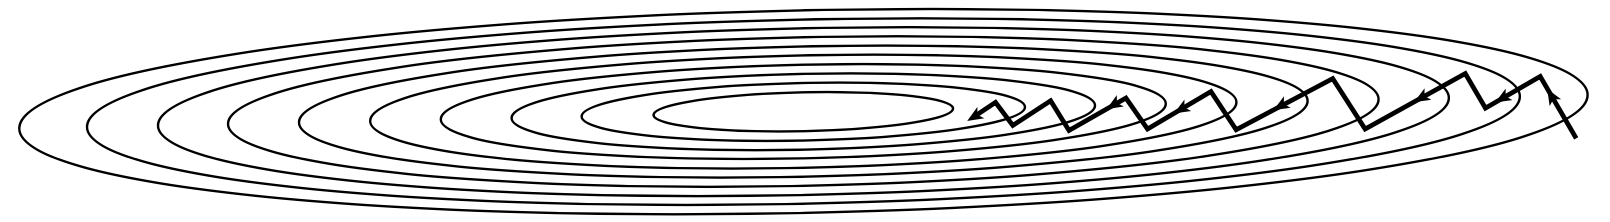
\includegraphics[width=\textwidth]{press_steepest_gradient_descent.png}
    \caption{Contour plot of the method of steepest gradient descent in a long, narrow valley \cite[421]{press1992}. Travel proceeds in near right angles due to the gradients.}
    \label{fig:gradient_descent_narrow_valley}
\end{figure}
Furthermore, if the step size is too large, the algorithm might `jump' over the ravine which poses an issue if the ravine contains the global minimum.
Per contra, DFO algorithms are not as sensitive to local noise, and their probing approach will facilitate more efficient progress along narrow valleys, although they will be more likely to accidentally jump over ravines if the step size is too large.

\chapter{Neural surfing theory}
\label{chap:neural_surfing_theory}
In the analogy of \ref{sec:motivation} we found that relying solely on our limited local information of the mountain landscape is not sufficient to effectively find the global minimum.
Luckily, in the case of neural networks, we actually have more information than just the error-weight surface.
This is the main idea behind the neural surfing technique. 
Instead of only considering the error-weight space, we will also look at the so-called output space. 
In doing so, we are viewing the neural training problem from a different perspective than it is classically studied. 
This chapter will discuss the concepts of weight and output space, as well as issues related to these concepts such as unrealisable regions and what is meant by a goal-connecting path.

\section{Weight and output spaces}
\label{sec:weight_and_output_spaces}
In \ref{def:mlp} we established that the tuple $\langle \mathscr{W}, \mathscr{B} \rangle$ along with the activation function is sufficient to fully define a MLP. 
Most importantly, we have $\mathscr{W} = \vec{W}_1, \vec{W}_2, \dots, \vec{W}_L$ and $\mathscr{B} = \vec{b}_1, \vec{b}_2, \dots, \vec{b}_L$ representing each layer's weight matrices and bias vectors, respectively. 
These parameters will be useful for defining the weight and ouput spaces.

\begin{definition}[Weight space]
    \label{def:weight_space}
    The weight space $\mathcal{W}_A$ of an artificial neural network $A$ is the set of all possible assignments to its \textit{trainable parameters}. 
    The trainable parameters are its weights $\mathscr{W}$ and biases $\mathscr{B}$.
    If $A$ has $P$ trainable parameters then its weight space is defined as
    \begin{equation}
        \mathcal{W}_A = \mathbb{R}^P.
    \end{equation}
\end{definition}

\begin{definition}[Output space]
    \label{def:output_space}
    The output space $\mathcal{O}_A$ of an artificial neural network $A$ with one output neuron spans the space of all possible output predictions on the training set.
    From \ref{eq:sup_learn_prediction}, the vector $\vec{\hat{y}}$ represents the prediction $\hat{y}$ for all $N$ training samples.
    The output space spans all possible assignments of $\vec{\hat{y}}$, so
    \begin{equation}
        \mathcal{O_A}=\mathbb{R}^N.
    \end{equation}
\end{definition}

\begin{lemma}
    \label{lmm:weight_space_sln}
    The weight space for a SLN $S$ with $m$ inputs and $n$ outputs is $\mathcal{W}_S = \mathbb{R}^{n(m+1)}$.
\end{lemma}
\begin{proof}
    $S$'s trainable parameters are the weight matrix $\vec{W} \in \mathbb{R}^{m\times n}$ from \ref{eq:sln_weight_matrix} and bias vector $\vec{b} \in \mathbb{R}^n$ from \ref{eq:sln_bias}.
    By \ref{def:weight_space}, the weight space encompasses all values of $\vec{W}$ and $\vec{b}$, so
    \begin{equation*}
        \mathcal{W}_S = \mathbb{R}^{m \times n} \times \mathbb{R}^{n} = \mathbb{R}^{m n + n} = \mathbb{R}^{(m + 1) n}.
    \end{equation*}
\end{proof}

\begin{lemma}
    \label{lmm:weight_space_mlp}
    A MLP $M$ with $L$ layers where the number of inputs to layer $l$ is given as $m_l$ will have the weight space $\mathcal{W}_M = \mathbb{R}^P$ where
    $P = \sum_{l=1}^{L-1}{\left(m_{l+1} (m_l + 1)\right)} + m_L + 1$.
\end{lemma}

\begin{proof}
    By \ref{def:mlp}, $M$ is comprised of $L$ SLNs which we will denote $\vec{S}_1, \vec{S}_2, \dots, S_L$.
    This allows us to express the weight space of $M$ as the product of the weight spaces of each of the SLNs,
    $$
        \mathcal{W}_M
        = \prod_{l=1}^L{\mathcal{W}_{S_l}}.
    $$

    For every layer $l$, the number of inputs to $S_l$ will be the number of inputs to the $l$th layer, $m_l$. 
    Let $n_l$ denote the number outputs for each layer $l$.
    Then, by \ref{lmm:weight_space_sln},
    $$\mathcal{W}_{S_l} = \mathbb{R}^{n_l(m_l+1)}.$$
    
    By splitting of the last factor in the product of weight spaces, we obtain 
    \begin{equation*}
        \mathcal{W}_M
        = \prod_{l=1}^{L-1}{\mathcal{W}_{S_l}} \times \mathcal{W}_{S_L}
        = \prod_{l=1}^{L-1}{\mathbb{R}^{n_l(m_l+1)}} \times \mathbb{R}^{n_L(m_L+1)}.
    \end{equation*}

    Notice that for any layer $l$, the number of outputs is equal to the number of inputs to the next layer, so $n_l=m_{l+1}$ except for the last layer where there is only one output unit leaving $n_L=1$.
    This leaves
    \begin{align*}
        \mathcal{W}_M
        &= \prod_{l=1}^{L-1}{\mathbb{R}^{m_{l+1}(m_l+1)}} \times \mathbb{R}^{m_L+1} \\
        &= \mathbb{R}^{\sum_{l=1}^{L-1}{m_{l+1}(m_l+1)}} \times \mathbb{R}^{m_L+1} \\
        &= \mathbb{R}^{\sum_{l=1}^{L-1}{m_{l+1}(m_l+1)} + m_L+1},
    \end{align*}
    so $\mathcal{W}_M = \mathbb{R}^P$ with
    \begin{equation*}
        P = \sum_{l=1}^{L-1}{m_{l+1}(m_l+1)} + m_L+1.
    \end{equation*}
\end{proof}

\begin{remark}
    The significance of \ref{lmm:weight_space_mlp} is that we obtain a formula for the number of trainable parameters $P$ in a MLP. 
    By \ref{def:weight_space}, $P$ determines the dimensionality of the weight space. 
    On other other hand, \ref{def:output_space} states that the number of samples in the training set $N$ determines the dimensionality of the output space.
    There is no relationship between $P$ and $N$ since the number of samples in the training set can be arbitrarily chosen. 
    It follows that there is no relationship between the dimensionalities of $\mathcal{W}$ and $\mathcal{O}$.
\end{remark}

\subsection{Relationship between weight and output space}
We will now examine the nature of the mapping between the two spaces, and whether there exists a linear mapping. 
Note that linear mappings can exist between spaces of different dimensionalities \cite{rudin2006}.

\begin{definition}[Weight-output mapping]
    \label{def:weight_output_space_mapping}
    Given an artifical neural network $A:\mathbb{R}^m \rightarrow \mathbb{R}^n$ with $m$ inputs and $n$ outputs parameterised by a set of trainable parameters $\vec{w} \in \mathcal{W_A}$,
    the weight-to-output-space mapping $h_A: \mathcal{W}_A \rightarrow \mathcal{O}_A$ for a dataset with $N$ $m$-dimensional feature vectors given by the matrix
    $\vec{X} = \begin{bmatrix}
        \vec{x}_1 & \vec{x}_2 & \cdots & \vec{x}_N
    \end{bmatrix}\tran \in \mathbb{R}^{N\times m}$
    is
    \begin{equation*}
        h_A \left( \vec{w} \right)
        = \begin{bmatrix}
            A(\vec{x}_1; \vec{w} ) \\
            A(\vec{x}_2; \vec{w} ) \\
            \vdots \\
            A(\vec{x}_N; \vec{w} ) \\
        \end{bmatrix}.
    \end{equation*}

    Note that we use the term `weight-output mapping' to refer to the `weight-to-output-space mapping' which should be confused with the mapping from weight space to a particular output prediction. 
\end{definition}

\begin{theorem}
    \label{thm:sln_one_output}
    For a SLN $S$ with one output unit, the function $h_S: \mathcal{W}_S \rightarrow \mathcal{O}_S$ is not a linear mapping.
\end{theorem}
\begin{proof}
    Let $S$ have $m$ inputs, as depicted in \ref{fig:sln_m_in_1_out}.
    Modifying the formula for a SLN given in \ref{def:sln} \ref{eq:single_layer_perceptron} for the case where there is only one output unit, we obtain
    $\hat{y} = f_\text{SLP}(\vec{x}; \vec{w}\tran, b) = g\left(\vec{w} \vec{x} + b\right)$
    where
    $\vec{x} = \begin{bmatrix}
        x_1 & x_2 & \cdots & x_m
    \end{bmatrix}\tran$
    is the input feature vector.

    We will consider a dataset with $N$ samples where the input is given by the $N\times m$ matrix
    $\vec{X} = \begin{bmatrix}
        \vec{x}_1 & \vec{x}_2 & \cdots & \vec{x}_N
    \end{bmatrix}\tran$
    as in \ref{eq:sup_learn_input_matrix}.
    By \ref{def:weight_output_space_mapping}, the mapping from weight to output space $h_S: \mathcal{W}_S \rightarrow \mathcal{O}_S$ is
    \begin{equation*}
        h_S \left( \vec{w} \right)
        = \begin{bmatrix}
            g \left( \vec{w}\tran \vec{x}_1 + b \right) \\
            g \left( \vec{w}\tran \vec{x}_2 + b \right) \\
            \vdots \\
            g \left( \vec{w}\tran \vec{x}_N + b \right) \\
        \end{bmatrix}.
    \end{equation*}

    We will assume, by way of contradiction, that $h$ is a linear mapping. 
    From the definition of linear mappings, it must be true that $h(\vec{u} + \vec{v}) = h(\vec{u}) + h(\vec{v})$ for $\vec{u}, \vec{v} \in \mathcal{W}_S$ \cite{rudin2006}.
    On the LHS we have
    \begin{equation*}
        h \left( \vec{u} + \vec{v} \right)
        = \begin{bmatrix}
            g((\vec{u} + \vec{v})\tran \vec{x}_1 + b) \\
            g((\vec{u} + \vec{v})\tran \vec{x}_2 + b) \\
            \vdots \\
            g((\vec{u} + \vec{v})\tran \vec{x}_N + b) \\
        \end{bmatrix}
        = \begin{bmatrix}
            g(\vec{u}\tran \vec{x}_1 + \vec{v}\tran \vec{x}_1 + b) \\
            g(\vec{u}\tran \vec{x}_2 + \vec{v}\tran \vec{x}_2 + b) \\
            \vdots \\
            g(\vec{u}\tran \vec{x}_N + \vec{v}\tran \vec{x}_N + b) \\
        \end{bmatrix}
    \end{equation*}
    and on the RHS we get
    \begin{equation*}
        h \left( \vec{u} \right) + h \left( \vec{v} \right)
        = \begin{bmatrix}
            g(\vec{u}\tran \vec{x}_1 + b) \\
            g(\vec{u}\tran \vec{x}_2 + b) \\
            \vdots \\
            g(\vec{u}\tran \vec{x}_N + b) \\
        \end{bmatrix}
        + \begin{bmatrix}
            g(\vec{v}\tran \vec{x}_1 + b) \\
            g(\vec{v}\tran \vec{x}_2 + b) \\
            \vdots \\
            g(\vec{v}\tran \vec{x}_N + b) \\
        \end{bmatrix}
        = \begin{bmatrix}
            g(\vec{u}\tran \vec{x}_1 + b) + g(\vec{v}\tran \vec{x}_1 + b) \\
            g(\vec{u}\tran \vec{x}_2 + b) + g(\vec{v}\tran \vec{x}_2 + b) \\
            \vdots \\
            g(\vec{u}\tran \vec{x}_N + b) + g(\vec{v}\tran \vec{x}_N + b) \\
        \end{bmatrix},
    \end{equation*}
    leaving
    \begin{equation*}
        \begin{bmatrix}
            g(\vec{u}\tran \vec{x}_1 + \vec{v}\tran \vec{x}_1 + b) \\
            g(\vec{u}\tran \vec{x}_2 + \vec{v}\tran \vec{x}_2 + b) \\
            \vdots \\
            g(\vec{u}\tran \vec{x}_N + \vec{v}\tran \vec{x}_N + b) \\
        \end{bmatrix}
        = \begin{bmatrix}
            g(\vec{u}\tran \vec{x}_1 + b) + g(\vec{v}\tran \vec{x}_1 + b) \\
            g(\vec{u}\tran \vec{x}_2 + b) + g(\vec{v}\tran \vec{x}_2 + b) \\
            \vdots \\
            g(\vec{u}\tran \vec{x}_N + b) + g(\vec{v}\tran \vec{x}_N + b) \\
        \end{bmatrix}.
    \end{equation*}

    Let $\alpha_i = \vec{u}\tran \vec{x}_i$ and $\beta_i = \vec{v}\tran \vec{x}_i$ for all $i$.
    Since $\vec{u},\vec{v} \in \mathbb{R}^m$ and all $\vec{x}_i \in \mathbb{R}^m$, it follows that $\alpha_i, \beta_i \in \mathbb{R}$ for all $i$.
    Hence $g(\alpha + \beta + b) = g(\alpha + b) + g(\beta + b)$.

    The only functions that satisfy $g$ are functions that satisfy Cauchy's functional equation\footnote{Cauchy's functional equation is $f(a+b)=f(a)+f(b)$. For $a,b \in \mathbb{Q}$, the only solutions are linear functions of the form $f(x) = cx$ for some $c \in \mathbb{Q}$ \cite{reem2017}.}, but these solutions only apply when $b=0$ and furthermore are linear, whereas the activation function $g$ is non-linear. 
    We arrived at a contradiction, thus disproving our initial assumption that $h$ is a linear mapping, so it must be a non-linear mapping.
\end{proof}

\begin{corollary}
    \label{col:weight_output_sln}
    For any SLN $S$, the function $h_S: \mathcal{W}_S \rightarrow \mathcal{O}_S$ is not a linear mapping.
\end{corollary}
\begin{proof}
    We will generalise the results from Theorem \ref{thm:sln_one_output} to SLNs with multiple outputs.
    Let $S$ have $m$ inputs and $n$ outputs.
    We construct $n$ smaller SLNs, $S_1,S_2,\dots,S_n$ where each $S_i$ has all $m$ input units, but only the $i$th output unit. 
    The DAG representing $S_i$ will only contain links from the input nodes to output node $\hat{y}_i$ (and, of course, the associated bias term $b_i$) as depicted in \ref{fig:sln_m_in_n_out_construction}.
    \begin{figure}
        \begin{center}
            \begin{tikzpicture}
                [
                    neuron/.style = {draw, circle, minimum size=25pt, inner sep=0pt, outer sep=0pt},
                ]
                
                \node [neuron] (x1)  at (0,0) {$x_1$};
                \node [neuron] (x2) at (0,-2) {$x_2$};
                \node (dots) at (0,-3) {$\vdots$};
                \node [neuron] (xm) at (0,-4) {$x_m$};
                \node [neuron,red] (y1) at (4,1) {$\hat{y}_1$};
                \node [neuron,green] (y2) at (4,-2) {$\hat{y}_2$};
                \node [neuron,blue] (yn) at (4,-5) {$\hat{y}_n$};
                \node [red] (b1) at (4, 2) {$b_1$};
                \node [green] (b2) at (4, -1) {$b_2$};
                \node [blue] (bn) at (4, -4) {$b_n$};
                \node (dots) at (4,-3.25) {$\vdots$};
                \draw[->,red] (x1) -- (y1);
                \draw[->,red] (x2) -- (y1);
                \draw[->,red] (xm) -- (y1);
                \draw[->,red] (b1) -- (y1);
                \draw[->,green] (x1) -- (y2);
                \draw[->,green] (x2) -- (y2);
                \draw[->,green] (xm) -- (y2);
                \draw[->,green] (b2) -- (y2);
                \draw[->,blue] (x1) -- (yn);
                \draw[->,blue] (x2) -- (yn);
                \draw[->,blue] (xm) -- (yn);
                \draw[->,blue] (bn) -- (yn);
            \end{tikzpicture}
        \end{center}
        \caption{The DAGs representing the constructions of $n$ SLNs with one output from a SLN with $m$ inputs and $n$ outputs. Each color represents one of the constructed smaller SLNs.}
        \label{fig:sln_m_in_n_out_construction}
    \end{figure}
    
    Now, we can simulate the function of $S$ by the construction
    \begin{equation*}
        S(\vec{x})
        = \begin{bmatrix}
            \hat{y}_1 \\
            \hat{y}_2 \\
            \vdots \\
            \hat{y}_n
        \end{bmatrix}
        = \begin{bmatrix}
            S_1(\vec{x}) \\
            S_2(\vec{x}) \\
            \vdots \\
            S_n(\vec{x})
        \end{bmatrix}.
    \end{equation*}
    By Theorem \ref{thm:sln_one_output}, each $S_i$ does not have a linear mapping from weight space to output space, so $S$ cannot have a linear mapping either.
\end{proof}

\begin{corollary}[Weight-output mapping in general]
    \label{col:weight_output_mlp}
    For any MLP $M$, $h_M: \mathcal{W}_M \rightarrow \mathcal{O}_M$ is not a linear mapping.
\end{corollary}
\begin{proof}
    Let $M$ have $L$ layers.
    By \ref{def:mlp}, $M$ is a nested function of $L$ SLNs. 
    \ref{col:weight_output_sln} states that each of these SLNs does not have a linear mapping from weight to output space.
    Hence the composition of $L$ SLNs that forms $M$ does not have a linear mapping from weight to output space.
\end{proof}

\begin{remark}
    The findings from \ref{col:weight_output_mlp} are very significant.
    They show that there is no apparent relationship between weight and output space that we can easily determine analytically. 
    If there were a straightforward mapping between weight and output space, we would be able to simply determine the ideal weight configuration that would achieve our target $\vec{y}$ in output space. 
    
    However, since this is not possible, the findings above set the scene for the neural surfing technique. 
    One of the core assumptions is that at a small enough scale, the mapping between weight and output space is \textit{locally linear}, or at least close enough.
\end{remark}

\subsection{Gradient descent from the perspective of weight and output space}
Gradient descent with mean squared error is classically viewed from the perspective of the error-weight surface. 
In this regard, its objective is to descend the error-weight surface.
Now that we have examined the relationship between the weight and output spaces, it follows naturally to determine how gradient descent fits in this frame of reference.
It becomes apparent that in output space, MSE can be thought of as greedily trying to reduce the Euclidean distance from $\vec{\hat{y}}$ to $\vec{y}$, i.e. from the prediction to the target.
To see this, recall \ref{def:mean_squared_error} and substitute
\begin{equation*}
    \norm{\vec{\hat{y}}-\vec{y}}=\sqrt{\sum_{i=1}^N{\left(\hat{y}_i - y_i\right)^2}}
\end{equation*}
in \ref{eq:mean_squared_error} to obtain
$
    E\left( \vec{y}, \vec{\hat{y}} \right) = \frac{1}{N} \norm{\vec{\hat{y}}-\vec{y}}^2
$. Since the number of samples $N$ is constant during training, there exists a linear relationship between the mean squared error and the Euclidean distance of the current output to the target output (goal).

\section{Unrealisable regions}
\begin{definition}[Strongly unrealisable point]
    \label{def:unrealisable_point}
    Given an artificial neural network $A$, a point $\vec{p} \in \mathcal{O}_A$ in output space is \textit{strongly unrealisable} if and only if there exists no weight configuration $\vec{w} \in \mathcal{W}_A$ such that $h_A(\vec{w}) = \vec{p}$.
    In order words, it is impossible to attain $\vec{p}$.
\end{definition}
\begin{definition}[Strongly unrealisable region]
    \label{def:unrealisable_region}
    Given an artificial neural network $A$, a \textit{strongly} unrealisable region $\mathcal{U} \subset \mathcal{O}_A$ is a subspace of the output space where every point $\vec{p} \in \mathcal{U}$ is strongly unrealisable.
    
    It is apparent that there exists no neural learning algorithm that can elicit a change in weight space that will attain a point in a strongly unrealisable region in output space.
    Hence we define a \textit{weakly} unrealisable region for a particular neural learning algorithm as a region in output space that cannot be attained by a particular algorithm.
\end{definition}

\begin{lemma}
    A strongly unrealisable region cannot encompass the whole output space.
\end{lemma}
\begin{proof}
    Let us consider an artifical neural network $A$. 
    We will show that for every unrealisable region, $\mathcal{U} \subsetneq \mathcal{O}_A$.
    By \ref{def:unrealisable_region}, $\mathcal{U} \subset \mathcal{O}_A$, so it remains to prove that every unrealisable region $\mathcal{U} \neq \mathcal{O}_A$.

    Choose any weight configuration $\vec{w} \in \mathcal{W}_A$. 
    Let the point $\vec{p}=h_A(\vec{w})$. 
    We know that $\vec{p}$ is \textit{not} strongly unrealisable because $\vec{w}$ achieves $\vec{p}$. 
    Hence no unrealisable region can contain $\vec{p}$, so $\vec{p} \notin \mathcal{U}$ but $\vec{p} \in \mathcal{O}_A$. 
    It follows that $\mathcal{U} \neq \mathcal{O}_A$.
\end{proof}

Let us look at a couple of examples of unrealisable regions.
\begin{example}
    \label{ex:unrealisable_trivial}
    A trivial example of an unrealisable region is predicting two different outputs for the same training sample.
    Consider again an MLP $M$ with one layer and two inputs, as shown in \ref{fig:sln_2_in_1_out}.
    Let $\vec{x}\in \mathbb{R}^2$ be any point in input space.
    For this example, let the training data be the matrix
    $
        \vec{X} = \begin{bmatrix}
            \vec{x} & \vec{x}
        \end{bmatrix}\tran
    $.
    Now we can define an unrealisable region
    \begin{equation*}
        \mathcal{U} = \left\{
            \begin{bmatrix}
                p_1 \\ p_2
            \end{bmatrix} : p_1, p_2 \in \mathbb{R}, p_1 \neq p_2
        \right\}
    \end{equation*}
    because $h_M(\vec{x})$ cannot produce two different outputs for the same value of $\vec{x}$.
\end{example}
\begin{example}[XOR mapping]
    \label{ex:unrealisable_xor}
    Let us look at a less contrived example.
    While it ``is well known that any Boolean function \elide can be approximated by a suitable two-layer feed-forward network'' \cite{blum1989}, 
    single-layer networks with non-decreasing activation functions can only learn a Boolean mapping that is \textit{linearly separable} \cite[723]{russell2010}.
    A linearly separable mapping has a linear decision boundary which means that there is only one linear hyperplane separating the two classes (true and false).
    
    The XOR function is not linearly separable because it requires at least two linear decision boundaries, as shown in \ref{fig:xor}.
    \begin{figure}
        \centering
        \begin{tikzpicture}
            \begin{axis}[
                x=2cm,
                y=2cm,
                axis lines=center,
                xlabel={$x_1$}, xlabel style={anchor=west},
                ylabel={$x_2$}, ylabel style={anchor=south},
                ymin=0, ymax=1.7,
                xmin=0, xmax=1.7,
                samples=100,
                xtick={0, 1},
                ytick={0, 1},
                extra x ticks=0,
                extra x tick style={
                    tick label style={
                        anchor=north east,
                        xshift=-.5*\pgfkeysvalueof{/pgfplots/major tick length}
                }}
            ]
                \addplot[black,only marks,mark=*] coordinates {(0,1) (1,0)};
                \addplot[black,only marks,mark=o] coordinates {(0,0) (1,1)};
                \addplot[black, no marks] coordinates {(0,.5) (.5,0)};
                \addplot[black, no marks] coordinates {(0,1.5) (1.5,0)};
                \addplot[black, ->] coordinates {(.25,.25) (.35,.35)};
                \addplot[black, ->] coordinates {(.75,.75) (.65,.65)};
            \end{axis}
        \end{tikzpicture}
        \caption{The locations of the two hyperplanes in input space acting as decision boundaries required to learn an XOR mapping. The filled-in dot represents an activation of 1 (true) and the circle represents 0 activation (false).}
        \label{fig:xor}
    \end{figure}
    We will consider the same single-layer architecture from \ref{fig:sln_2_in_1_out} again, using the sigmoid activation function.
    The sigmoid is a non-decreasing function.
    Since we only have one unit (the output neuron) with this non-decreasing non-linear activation function, it follows that we can only have one decision boundary.
    We just showed that the XOR mapping requires two decision boundaries.
    Therefore, given the input matrix
    \begin{equation*}
        \vec{X} = \begin{bmatrix}
            0 & 0 \\
            0 & 1 \\
            1 & 0 \\
            1 & 1
        \end{bmatrix},
    \end{equation*}
    the point
    $
        \vec{p} = \begin{bmatrix}
            0 & 1 & 1 & 0
        \end{bmatrix}\tran
    $
    in output space is strongly unrealisable.
    So $\mathcal{U} = \{\vec{p}\}$ is an example of an unrealisable region.    
\end{example}

\begin{remark}
    \ref{ex:unrealisable_trivial,ex:unrealisable_trivial} demonstrate that unrealisable regions can arise even in very simple scenarios, so it is vital to take this phenomenon into account when designing a path-finding technique in output space, such as the neural surfer.
    Furthermore, one must also consider what happens if the target $\vec{y}$ lies in an unrealisable region (which means that $\vec{y}$ itself is unrealisable).
    In this case, the global minimum of the error-weight surface (using mean squared error) would be the weight configuration that produces the point closest to $\vec{y}$ (in terms of Euclidean distance) which is realisable.
\end{remark}

\section{Goal-connecting paths}
\begin{definition}[Goal-connecting path]
    \label{def:goal_connecting_path}
    For an artificial neural network $A$ with current weight configuration $\vec{w}_0 \in \mathcal{W}_A$, a goal-connecting path in output space to the goal $\vec{g}\in \mathcal{O}_A$ is a sequence of points $\vec{s}_0, \vec{s}_1,\dots,\vec{s}_{S} \in \mathcal{O}_A$ where the initial state $\vec{s}_0 = h_A(\vec{w}_0)$ and final state $\vec{s}_S=\vec{g}$.
    The points $\vec{s}_1,\vec{s}_2,\dots,\vec{s}_S$ are referred to as \textit{subgoals}, hence $S$ is the number of subgoals in the goal-connecting path. 

    The goal-connecting path is \textit{realizable} if and only if no subgoal is a strongly unrealisable point (\ref{def:unrealisable_point}).
    This means that a realizable goal-connecting path can equivalently be defined by the weight configurations $\vec{w}_0, \vec{w_1},\dots,\vec{w}_S \in \mathcal{W}_A$ such that $h_A(\vec{w}_i) = \vec{s}_i$ for $i \leq S$.
\end{definition}

\begin{definition}[Ideal goal-connecting path]
    \label{def:ideal_goal_connecting_path}
    The ideal goal-connecting path of $S$ subgoals for an artifical neural network $A$ is, in terms of weight space, the \textit{shortest} realizable goal-connecting path with equidistant subgoals. 
\end{definition}

\begin{lemma}
    \label{lmm:ideal_subgoal_construction}
    Given $\vec{w}_0$ and $\vec{w}_S$, the $i$th subgoal of the ideal goal-connecting path in weight space is given by
    $
        \vec{w}_i = \vec{w}_0 + \frac{i}{S}\left( \vec{w}_S - \vec{w}_0 \right)
    $.
\end{lemma}
\begin{proof}
    First, we will show that the points are equidistant, i.e. $\norm{\vec{w}_0 - \vec{w}_1} = \norm{\vec{w}_1 - \vec{w}_2} = \dots = \norm{\vec{w}_{S-1} - \vec{w}_S}$.
    This is equivalent to asserting that $\norm{\vec{w}_{i-1} - \vec{w}_i} = \norm{\vec{w}_i - \vec{w}_{i+1}}$ for $0 < i < S$.
    Substituting on the LHS,
    \begin{align*}
        \norm{\vec{w}_{i-1} - \vec{w}_i}
        &= \norm{\vec{w}_0 + \frac{i-1}{S}\left( \vec{w}_S - \vec{w}_0 \right) - \vec{w}_0 - \frac{i}{S}\left( \vec{w}_S - \vec{w}_0 \right)} \\
        &= \norm{-\frac{1}{S}\left(\vec{w}_S - \vec{w}_0 \right)},
    \end{align*}
    and on the RHS,
    \begin{align*}
        \norm{\vec{w}_i - \vec{w}_{i+1}}
        &= \norm{\vec{w}_0 + \frac{i}{S}\left( \vec{w}_S - \vec{w}_0 \right) - \vec{w}_0 - \frac{i+1}{S}\left( \vec{w}_S - \vec{w}_0 \right)} \\
        &= \norm{-\frac{1}{S}\left(\vec{w}_S - \vec{w}_0 \right)}.
    \end{align*}

    The shortest path between two points is a straight line, so the ideal goal-connecting path in weight space must form a straight line from $\vec{w}_0$ to $\vec{w}_S$, and all subgoals must lie on this line.
    The equation of the line $l:\mathbb{R} \rightarrow \mathcal{W}_A$ from $\vec{w}_0$ to $\vec{w}_S$ is $l(\lambda) = \vec{w}_0 + \lambda\left( \vec{w}_S - \vec{w}_0 \right)$.
    It is easy to see that $l\left(\frac{i}{S}\right)=\vec{w}_i$ for $0 \leq i \leq S$, so the subgoals are collinear.
\end{proof}

\begin{remark}
    \ref{lmm:ideal_subgoal_construction} shows a construction for achieving the ideal goal-connecting path, given knowledge of the target weight configuration $\vec{w}_S$.
    Of course, this is not known to the neural learning algorithm while it is learning, only once it finished and was able to actually achieve the goal. 
    However, we can use the ideal goal-connecting path in retrospect to evaluate the performance of the neural learning algorithm in comparison to the ideal path.
    Furthermore, we can plot the ideal goal-connecting path in output space in order to find unrealisable regions.
\end{remark}

\section{A `cheat' technique for evaluating subgoal trajectories}
\label{sec:cheating_technique}
The neural surfer must be able to perform two main tasks: 
\begin{enumerate*}[label=(\roman*)]
    \item set the subgoals in output space; and
    \item achieve these subgoals.
\end{enumerate*}
This `cheat' technique pertains only to the latter task, ignoring the former.
It can be used in order to determine whether and to what extent a training regime\footnote{This technique can be used for \textit{any} regime that provides a mechanism for achieving (sub)goals. As such, this technique not only provides a means of testing the neural surfing algorithm, but also provides a means of using gradient to realise a subgoal trajectory.} is \textit{capable} of realising each subgoal.
The idea is that splitting the problem into two parts will facilitate a better analysis of the neural surfing technique by isolating pain points and performance issues.
Two main questions can be evaluated:
\begin{itemize}
    \item How well is the approach getting to the subgoals?
    \item How good is the state the approach ends up in when it achieves the subgoal?
\end{itemize}

\paragraph{Achieving a subgoal}
One important question that must be answered is what constitutes realising a subgoal. 
For the purpose of this technique, we will assume that achieving some fraction $\mu\in(0,1)$ of the distance to the subgoal constitutes as `achieving' it. 
In more sophisticated scenarios, this technique could be extended to use functions that give a specific threshold for each subgoal.

\paragraph{Procedure}
The steps below explain the methodology of this technique, for $S$ subgoals (where the last subgoal represents the goal).
\begin{figure}
    \centering
    \begin{tikzpicture}
        \begin{axis}[
            scale only axis,
            width=.6\textwidth,
            height=.4\textwidth,
            xmin=0, xmax=15,
            ymin=0, ymax=10,
            xlabel={$\hat{y}_1$},
            ylabel={$\hat{y}_2$},
            ticks=none,
            axis x line=bottom,
            axis y line=left
        ]
            \coordinate (initial) at (2, 4);
            \coordinate (goal) at (12.5, 7.5);
            \coordinate (y1) at (4, 1);
            \coordinate (y2) at (7, 1);
            \coordinate (y3) at (10, 5);

            \draw[->] (initial) (initial) to[curve through={(y1) .. (y2) .. (y3)}] (goal);

            \node[label={180:{$\vec{\hat{y}}_0$}}, circle, fill, inner sep=1pt] at (initial) {};
            \node[label={270:{$\vec{\hat{y}}_1$}}, circle, fill, inner sep=1pt] at (y1) {};
            \node[label={90:{$\vec{\hat{y}}_2$}}, circle, fill, inner sep=1pt] at (y2) {};
            \node[label={180:{$\vec{\hat{y}}_3$}}, circle, fill, inner sep=1pt] at (y3) {};
            \node[label={90:{$\vec{\hat{y}}_4$}}, circle, fill, inner sep=1pt] at (goal) {};

            \draw
                let
                    \p1 = ($(y1) - (initial)$),
                    \p2 = ($(y2) - (y1)$),
                    \p3 = ($(y3) - (y2)$),
                    \p4 = ($(goal) - (y3)$),
                    \n1 = {veclen(\x1, \y1)/2},
                    \n2 = {veclen(\x2, \y2)/2},
                    \n3 = {veclen(\x3, \y3)/2},
                    \n4 = {veclen(\x4, \y4)/2}
                in
                    (y1) circle (\n1)
                    (y2) circle (\n2)
                    (y3) circle (\n3)
                    (goal) circle (\n4);
            
            \draw[dashed]
                (initial) -- (y1)
                (y1) -- (y2)
                (y2) -- (y3)
                (y3) -- (goal);
        \end{axis}
    \end{tikzpicture}
    \caption{Output space for the `cheat' technique for $S=4$ subgoals and $\mu=\frac{1}{2}$. The circles around each point indicate the threshold that constitutes `achieving' a particular point. The radius of the circle around point $\vec{\hat{y}}_i$ is $(1-\mu) \norm{\vec{\hat{y}}_i-\vec{\hat{y}}_{i-1}}$ for $i=1, \dots, S$; hence the circles are not necessarily identical in size. While the weight configurations $\vec{w}_0, \dots, \vec{w}_S$ are equidistant and collinear in weight space, it is important to note that the corresponding points in output space $\vec{y}_1, \dots, \vec{y}_{n+1}$ will usually neither be collinear nor equidistant due to the inherent non-linearity of the network. In practice, $\mu$ will be set to a larger value such as $0.9$ (which will decrease the circles' radii) to ensure that enough progress was made in achieving a subgoal before proceding to the next.}
    \label{fig:cheat_technique}
\end{figure}
\ref{fig:cheat_technique} illustrates this technique in output space.
\begin{enumerate}
    \item Determine the point in weight space $\vec{w}_S$ that corresponds to the target in output space (i.e. the global minimum on the error-weight surface). 
        
        This can be done either by
        \begin{enumerate*}[label=(\roman*)]
            \item analytically finding the global minimum of the error-weight space if the network architecture is simple enough (see \ref{thm:stripe_global_minima}); or
            \item running gradient descent from many random initial configurations in order to find the (likely) global minimum.
        \end{enumerate*}
    
    \item Determine the ideal goal line $\vec{w}_1,\vec{w}_2,\dots,\vec{w}_S$ in weight space using \ref{lmm:ideal_subgoal_construction} and the corresponding goal-connecting path $\vec{\hat{y}}_1,\vec{\hat{y}}_2,\dots,\vec{\hat{y}}_S$ in output space.
    \item Let $i=0$. Starting at weight configuration $\vec{w}_i$, perform the particular neural network training technique until achieving a point $\vec{p}$ in output space where $\norm{\vec{p} - \vec{\hat{y}}_{i+1}} \leq (1-\mu) \norm{\vec{\hat{y}}_i - \vec{\hat{y}}_{i+1}}$, i.e. at least a fraction $\mu$ of the distance to the next subgoal is achieved.
    \item Repeat the previous step for $i=1, 2, \dots, S$.
\end{enumerate}
We will employ this technique in \ref{sec:stripe_gradient_descent_subgoals,sec:stripe_derivative_free_subgoals} to evaluate the feasability of the ideal goal line in a suboptimal local minimum setting using both gradient-based and derivative-free optimisation regimes.

\chapter{The local minimum problem}
\label{chap:local_minimum_problem}
The previous chapters explained the theory behind neural networks and their classical training algorithms. 
We looked at some of these algorithms' shortcomings in \ref{sec:neural_training_issues} and hypothesised why they would potentially fail to find global minima in the presence of suboptimal local minima.
Now we can define the local minimum problem more accurately, contrive an example of said problem, and finally not only analyse it from the classical viewpoint of \ref{chap:neural_network_theory}, but also relate it to the paradigm of \ref{chap:neural_surfing_theory}.

\section{The mathematics of local and global minima}
In order to contrive and analyse an instance of the local minimum problem, we must formally define what is meant by `local' and `global' minima and identify the necessary and sufficient conditions that prove their existence.
We will do this by returning to the running analogy of hiking in the mountains to provide some intuition.
Let us begin with the global minimum, which is simply a point with an elevation lower than any other point.
\begin{definition}[Global minimum]
    \label{def:global_minimum}
    The function $f: \mathbb{R}^n \rightarrow \mathbb{R}$ has a \textit{global minimum} at point
    $\vec{p} \in \mathbb{R}^n$
    if and only if for all
    $\vec{x} \in \mathbb{R}^n$
    it is true that
    $f(\vec{p}) \leq f(\vec{x})$.
\end{definition}

We claimed in \ref{sec:motivation} to have a local minimum if the surroundings of our one-metre radius of vision are of higher elevation than the ground beneath our feet.
To define local minima, we will use the same concept, just allowing that the radius of the circle describing the visible surroundings can be arbitrarily small.
\begin{definition}[Local minimum]
    \label{def:local_minimum}
    The function $f: \mathbb{R}^n \rightarrow \mathbb{R}$ has a \textit{local minimum} at point
    $\vec{p} \in \mathbb{R}^n$
    if there exists a ball with centre
    $\vec{p}$
    where
    $f(\vec{p}) \leq f(\vec{x})$
    for all points $\vec{x}$ in that ball.
    A \textit{suboptimal local minimum} is a local minimum that is not a global minimum.
\end{definition}

Now it is possible to define the local minimum problem using these terms.
\begin{problem}[Local minimum problem]
    A training algorithm exhibits the local minimum problem if there exists a weight initialisation that leads to training converging to a suboptimal local minimum on the error-weight surface.

    This problem arises when a gradient-based agent is initialised in a valley with a suboptimal local minimum, i.e. it is initialised at a weight configuration where following the gradients will ultimately lead to a suboptimal local minimum.
\end{problem}

In order to later examine error-weight surfaces analytically, we must derive the conditions that are necessary and sufficient for local minima to exist.
We must first realise that if our immediate surroundings are of higher elevation, then the infinitesimal slope beneath our feet is completely flat (because moving just a bit in any direction will lead to a higher elevation). 
In formal terms, this infinitesimal slope is the gradient, or vector of first partial derivatives, which is given by the \textit{Jacobian}.
\begin{definition}[Jacobian]
    Let $f: \mathbb{R}^n \rightarrow \mathbb{R}$ be a continuously differentiable function of the form
    $f=f\left(\vec{x}\right)$
    where
    $\vec{x} = \begin{bmatrix}
        x_1 & x_2 & \cdots & x_n
    \end{bmatrix}\tran$.
    The Jacobian of $f$ (or simply \textit{derivative} of $f$) is a row vector of its first-order partial derivatives,
    \begin{equation*}
        \vec{J}_f
        = \frac{\delta f}{\delta \vec{x}}
        = \begin{bmatrix}
            \frac{\delta f}{\delta x_1} &
            \frac{\delta f}{\delta x_2} &
            \cdots &
            \frac{\delta f}{\delta x_n}
        \end{bmatrix}.
    \end{equation*}
\end{definition}

Now that we have defined the Jacobian as representing the infinitesimal slope of the mountain, we must realise an important fact.
Knowing that the slope of the mountain is flat at a specific point is not a sufficient condition for there being a local minimum; after all, we could be talking about a global maximum (or a saddle point).
We will call these points \textit{critical points}.
To determine whether a critical point constitutes a local minimum, we must examine its immediate surrounding, to see if these points are of higher elevation.
This will be achieved by looking at the second partial derivatives given by the \textit{Hessian}, more specifically the existence of a local minima is predicated on whether the Hessian is \textit{positive definite}.
Let us define these terms.
\begin{definition}[Hessian]
    Let $f: \mathbb{R}^n \rightarrow \mathbb{R}$ be a function of the form
    $f=f\left(\vec{x}\right)$
    where
    $\vec{x} = \begin{bmatrix}
        x_1 & x_2 & \cdots & x_n
    \end{bmatrix}\tran$
    for which all second partial derivatives exist and are continuous over $\mathbb{R}^n$.
    The Hessian of $f$ is a $n\times n$ matrix of the second-order partial derivatives, given by
    \begin{equation*}
        \vec{H}_f = \begin{bmatrix}
            \frac{\delta^2 f}{\delta x_1^2} &
            \frac{\delta^2 f}{\delta x_1 x_2} &
            \cdots &
            \frac{\delta^2 f}{\delta x_1 x_n} \\
            \frac{\delta^2 f}{\delta x_2 x_1} &
            \frac{\delta^2 f}{\delta x_2^2} &
            \cdots &
            \frac{\delta^2 f}{\delta x_2 x_n} \\
            \vdots & \vdots & \ddots & \vdots \\
            \frac{\delta^2 f}{\delta x_n x_1} &
            \frac{\delta^2 f}{\delta x_n x_2} &
            \cdots &
            \frac{\delta^2 f}{\delta x_n^2}
        \end{bmatrix}.
    \end{equation*}
\end{definition}
\begin{definition}[Positive definite matrix]
    \label{def:positive_definite}
    A symmetric $n\times n$ matrix $\vec{M} \in \mathbb{R}^{n\times n}$ is said to be \textit{positive definite} if and only if
    $\vec{x}\tran \vec{M} \vec{x} > 0$
    for all $\vec{x} \in \mathbb{R}^n \setminus \vec{0}$.
\end{definition}
We will prove a simple technique for showing that a $2 \times 2$ matrix is positive definite, as this will help us prove the existence of local minima later.
\begin{theorem}[$2\times 2$ positive definite matrix]
    \label{thm:positive_definite_2_by_2}
    The matrix $\vec{M} = \begin{bmatrix}
        a & b \\ b & c
    \end{bmatrix}$
    is positive definite if
    $a > 0$ and 
    $ac - b^2>0$.
\end{theorem}
\begin{proof}
    Let $\vec{x} = \begin{bmatrix}
        x_1 & x_2
    \end{bmatrix}\tran$
    and $f(x_1, x_2) = \vec{x}\tran \vec{M} \vec{x}$.
    Performing the multiplication,
    \begin{align*}
        f(x_1, x_2)
        &= 
        \begin{bmatrix}
            x_1 & x_2
        \end{bmatrix}
        \begin{bmatrix}
            a & b \\
            b & c
        \end{bmatrix}
        \begin{bmatrix}
            x_1 \\ x_2
        \end{bmatrix} \\
        &=
        \begin{bmatrix}
            x_1 a + x_2 b & x_1 b + x_2 c
        \end{bmatrix}
        \begin{bmatrix}
            x_1 \\ x_2
        \end{bmatrix} \\
        &=
            x_1^2 a + 2 x_1 x_2 b + x_2^2 c.
    \end{align*}

    We will now discuss under what conditions
    $f(x_1, x_2) > 0$
    holds.
    When $x_2=0$, it must necessarily be the case that $a>0$.
    Otherwise, dividing by $x_2^2$, we can write
    \begin{align*}
        \left(\frac{x_1}{x_2}\right)^2 a + \frac{2 x_1 b}{x_2} + c > 0,
    \end{align*}
    and substituting $p = \frac{x_1}{x_2}$ we get
    \begin{align*}
        p^2 a + 2pb + c > 0.
    \end{align*}
    Treating this as a quadratic function in terms of $p$, we realise that since $a>0$, the parabola opens up.
    The discriminant $D=4b^2 - 4ac$ is negative if $ac-b^2>0$ which means that the parabola has no roots. 
    Thus its range is positive.

    We have shown that $f(x_1, x_2)>0$ if $a>0$ and $ac-b^2>0$ for all $x_1,x_2\in \mathbb{R}$ except $x_1=x_2=0$.
    By \ref{def:positive_definite}, $\vec{M}$ must be positive definite.
\end{proof}

Let us finally introduce a theorem that we can later use as a tool to prove the existence of local minima.
\begin{theorem}[Local minimum]
    Let $f: \mathbb{R}^n \rightarrow \mathbb{R}$ be a continuously differentiable function, and let the point
    $\vec{p} \in \mathbb{R}^n$
    be such that
    $\vec{J}_f(\vec{p}) = \vec{0}$
    and
    $\vec{H}_f(\vec{p})$ is positive definite.
    Then $\vec{p}$ is a \textit{local minimum} of $f$.
\end{theorem}
We will require this theorem to justify that gradient-based training converges to a local minimum in \ref{sec:stripe_problem}.
However, the proof of this theorem exceeds the scope of this report.
The interested reader may consult \textcite[190]{loomis1990}.

\section{The stripe problem}
\label{sec:stripe_problem}
The local minimum problem has been studied with regard to sigmoidal MLPs with one hidden layer by \textcite{blum1989}.
Amongst others, \citeauthor{blum1989} proved the existence of suboptimal local minima in certain configurations. 

The so-called \textit{stripe problem}, as given by \textcite{weir2019} is a practical example of how local minima arise in a 2-2-1 sigmoidal MLP.
Consider a two-dimensional input space with two initially parallel hyperplanes that form a stripe.
The initial configuration will have the hyperplanes arranged horizontally and misclassify some of the samples. 
Changing the weights in the neural network will allow the hyperplanes to rotate, but when they do so, they are forced to misclassify even more samples (thereby increasing the mean squared error) until eventually reaching the target configuration with zero error.
\ref{fig:stripe_original_hyperplanes} shows the initial and target configurations of the hyperplanes for this type of network.
The hidden layer is required because without it, the sigmoid activation function will produce only one hyperplane, as proved in \ref{lmm:sigmoid_decision_boundary}.
\begin{figure}
    \centering
    \begin{subfigure}{.45\textwidth}
        \begin{tikzpicture}
            \begin{axis}[
                x=1cm,
                y=1cm,
                axis lines=center,
                xlabel={$x_1$}, xlabel style={anchor=west},
                ylabel={$x_2$}, ylabel style={anchor=south},
                ymin=0, ymax=4,
                xmin=0, xmax=4,
                enlargelimits={upper},
                grid=none,
                samples=100,
                ticks=none
            ]
                \addplot[black,only marks,mark=*] coordinates {(2,1.5) (2,2.5)};
                \addplot[black,only marks,mark=o] coordinates {(2,.5) (.5,.5) (3.5,.5) (.5,3.5) (3.5,3.5) (2,3.5)};
                \addplot[black, no marks] coordinates {(0,1) (4,1)};
                \addplot[black, no marks] coordinates {(0,3) (4,3)};
                \addplot[black, ->] coordinates {(1,1) (1,1.35)};
                \addplot[black, ->] coordinates {(1,3) (1,2.65)};
            \end{axis}
        \end{tikzpicture}
        \caption{Initial configuration}
    \end{subfigure}
    \hspace*{\fill}
    \begin{subfigure}{.45\textwidth}
        \begin{tikzpicture}
            \begin{axis}[
                x=1cm,
                y=1cm,
                axis lines=center,
                xlabel={$x_1$}, xlabel style={anchor=west},
                ylabel={$x_2$}, ylabel style={anchor=south},
                ymin=0, ymax=4,
                xmin=0, xmax=4,
                enlargelimits={upper},
                grid=none,
                samples=100,
                ticks=none
            ]
                \addplot[black,only marks,mark=*] coordinates {(2,.5) (2,1.5) (2,2.5) (2,3.5)};
                \addplot[black,only marks,mark=o] coordinates {(.5,.5) (3.5,.5) (.5,3.5) (3.5,3.5)};
                \addplot[black, no marks] coordinates {(1,0) (1,4)};
                \addplot[black, no marks] coordinates {(3,0) (3,4)};
                \addplot[black, ->] coordinates {(1,1) (1.35,1)};
                \addplot[black, ->] coordinates {(3,1) (2.65,1)};
            \end{axis}
        \end{tikzpicture}
        \caption{Target configuration}
    \end{subfigure}
    \caption{Hyperplanes in input space for the stripe problem with eight samples (adapted from \textcite{weir2019}).}
    \label{fig:stripe_original_hyperplanes}
\end{figure}

In this section, we will formulate a version of the stripe problem that requires no hidden layers and fewer input samples by using a different kind of activation function.
The reduced number of parameters will lend itself better for analysis.

\subsection{Radial basis activation functions}
We will first introduce the concept of radial basis functions. 
When used as the activation function, they exhibit some advantageous properties that will aid us to contrive a simple version of the stripe problem.
\begin{definition}[Radial basis function]
    \label{def:rbf}
    A radial basis function (RBF) is a smooth continuous real-valued\footnote{We define RBFs has having a scalar domain and range because this suffices for our purposes. In actual fact, RBFs are defined more generally to map between suitable vector spaces \cite{buhmann2000}.} function $\phi : \mathbb{R} \rightarrow \mathbb{R}$ that satisfies the property $\phi(x) = \phi(\norm{x})$ \cite{buhmann2000}. 
    %RBFs are commonly used as a kernel in support vector machines (SVMs) \cite{burkov2019}.
    For RBFs to be useful activation functions, we three additional restrictions:
    \begin{enumerate*}[label=(\roman*)]
        \item $\phi(0)=1$;
        \item $\phi(x)$ is strictly decreasing for the domain $[0, \infty)$ when $\phi(x) \neq 0$; and
        \item that
    \end{enumerate*}
    \begin{equation*}
        \lim_{x\rightarrow -\infty}{\phi(x)} = \lim_{x\rightarrow \infty}{\phi(x)} = 0.
    \end{equation*}
\end{definition}

Two commonly used RBFs, both infinitely differentiable, are the Gaussian function
\begin{equation}
    \label{eq:gaussian}
    \phi(x) = e^{-x^2}
\end{equation}
and the bump function\footnote{We give a slightly modified version of the well-known $C_\infty$ ``bump'' function \cite{johnson2015} that is vertically scaled such that $\phi(0)=1$ for convenience.}
\begin{equation}
    \label{eq:bump}
    \phi(x) = 
    \begin{cases}
        e^{1-\frac{1}{1-x^2}} & \text{for $-1<x<1$} \\
        0 & \text{otherwise}
    \end{cases}.
\end{equation}
These functions, graphed in \ref{fig:rbfs}, exhibit slightly different properties.
\begin{figure}
    \centering
    \begin{tikzpicture}[
        declare function={
            gaussian(\x)= exp(-\x^2);
            bump(\x)= and(\x>=-1, \x<=1) * exp(1-1/(1-(\x^2)));
        }
    ]
        \begin{axis}[
            x=1.5cm,
            y=1.5cm,
            axis lines=center,
            xlabel={$x$}, xlabel style={anchor=west},
            ylabel={$\phi(x)$}, ylabel style={anchor=south},
            ymin=0, ymax=2,
            xmin=-3, xmax=3,
            enlarge x limits={true,abs value=.2},
            enlarge y limits={upper,abs value=.2},
            grid,
            samples=100,
            xtick={-3,...,3},
            ytick={0, 1, 2},
            extra x ticks = 0
        ]
            \addplot[blue] {gaussian(x)};
            \addplot[red,domain=-1:1] {bump(x)};
            \legend{Gaussian function,bump function}
        \end{axis}
    \end{tikzpicture}
    \caption{Plots of the two most common radial basis functions.}
    \label{fig:rbfs}
\end{figure}
The Gaussian function never actually reaches zero and its derivative is never zero (except at the peak, i.e. $x=0$). 
On the other hand, for the bump function, we have $\phi(x)=0$ and $\frac{d\phi}{dx}=0$ for $x \notin (-1, 1)$.

\begin{lemma}[Single-layer RBF decision boundaries]
    \label{lmm:single_layer_rbf_decision_boundaries}
    A single-layer Gaussian RBF MLP with decision threshold $t\in (0,1)$ will have two hyperplanes in input space.
\end{lemma}
\begin{proof}
    The proof is similar in method as in \ref{lmm:sigmoid_decision_boundary}.
    Consider an equivalent SLN $S$ with $m$ inputs and one output as shown in \ref{fig:sln_m_in_1_out}. 
    To obtain the decision boundaries, we set the output equal to the decision threshold, so
    \begin{align*}
        t &= S\left(\vec{x}\right) \\
        &= \phi\left(\vec{w}\tran \vec{x} + b\right) \\
        &= e^{-\left(\vec{w}\tran \vec{x} + b \right)^2} \\
        -\ln{t} &= \left(\vec{w}\tran \vec{x} + b \right)^2 \\
        \pm \sqrt{-\ln{t}} &= \vec{w}\tran \vec{x} + b.
    \end{align*}
    Since $t\in (0,1)$, it follows that $\ln t < 0$ and thus $\sqrt{-\ln{t}} > 0$ which of course means that $\sqrt{-\ln{t}} \neq 0$. 
    Hence
    \begin{equation}
        \label{eq:gaussian_hyperplanes}
        \vec{w}\tran \vec{x} + b \pm \sqrt{-\ln{t}} = 0
    \end{equation}
    has two distinct solutions, no matter the values of $\vec{w}$, $\vec{x}$, and $b$.
    Thus there will always be two hyperplanes.
\end{proof}
\begin{remark}
    Although \ref{lmm:single_layer_rbf_decision_boundaries} proves the existence of two hyperplane decision boundaries for Gaussian RBFs, it is trivial to modify this proof for any other type of RBF, such as the bump function.
    As a consequence, we know that unlike single-layer sigmoidal networks (see \ref{lmm:sigmoid_decision_boundary}), we can use single-layer RBF networks to generate a decision boundary in the form of a stripe which will allow us to use this type of network to provide a more simple example of the stripe problem.
\end{remark}

\begin{example}
    \label{ex:sln_2_in_1_out_gaussian_hyperplanes}
    Like in \ref{ex:sln_2_in_1_out_sigmoid_hyperplane}, let us consider once more a single-layered MLP $M$ with two inputs, depicted in \ref{fig:sln_2_in_1_out}, where $w_1=w_2=1$ and $b=0$. 
    Let the threshold be $t=\frac{1}{2}$ again, but this time, we will use the Gaussian RBF as the activation function.

    From \ref{eq:gaussian_hyperplanes}, we obtain the equations of the hyperplanes as
    \begin{align*}
        \vec{w}\tran \vec{x} + b \pm \sqrt{-\ln{\frac{1}{2}}} &= 0 \\
        w_1 x_1 + w_2 x_2 + b &=  \pm \sqrt{-\ln{\frac{1}{2}}} \\
        x_1 + x_2 &= \pm \sqrt{-\ln{\frac{1}{2}}},
    \end{align*}
    so the hyperplanes are at $x_2 = -x_1 - 0.8325\dots$ and $x_2 = -x_1 + 0.8325\dots$, as shown in \ref{fig:gaussian_hyperplanes}.

    \begin{figure}
        \begin{subfigure}[b]{0.45\textwidth}
            \begin{tikzpicture}[
                declare function={
                    hminus(\x)= -\x - sqrt(-ln(0.5));
                    hplus(\x)= -\x + sqrt(-ln(0.5));
                }
            ]
                \begin{axis}[
                    scale only axis,
                    width=.8\textwidth,
                    axis lines=center,
                    xlabel={$x_1$}, xlabel style={anchor=west},
                    ylabel={$x_2$}, ylabel style={anchor=south},
                    ymin=-2.5, ymax=2.5,
                    xmin=-2.5, xmax=2.5,
                    samples=2
                ]
                    \addplot[black,only marks,mark=*] coordinates {(0,0) (-1,1) (1,-1)};
                    \addplot[black,only marks,mark=o] coordinates {(1,1) (-1, 2.2) (1.5,0) (0,1.5) (2.2,1) (1,2.2) (2.2,-1) (-1,-1) (1, -2.2) (-1.5,0) (0,-1.5) (-2.2,-1) (-1,-2.2) (-2.2,1)};
                    \addplot[black, no marks] {hminus(x)};
                    \addplot[black, no marks] {hplus(x)};
                    \addplot[black, ->] coordinates {(-2,{hminus(-2)}) (-1.75, {2*hminus(-2)-hminus(-1.75)})};
                    \addplot[black, ->] coordinates {({-hminus(-2)},{hplus(-hminus(-2))}) ({-hminus(-2)-.25}, {2*hplus(-hminus(-2))-hplus(-hminus(-2)-.25)})};
                \end{axis}
            \end{tikzpicture}
            \vspace{.5cm}
            \caption{Input space with sample data}
        \end{subfigure}
        \hspace*{\fill}
        \begin{subfigure}[b]{0.55\textwidth}
            \begin{tikzpicture}
                \begin{axis}[
                    scale only axis,
                    width=.7\textwidth,
                    ymin=-3, ymax=3,
                    xmin=-3, xmax=3,
                    zmin=0, zmax=1,
                    xlabel={$x_1$},
                    ylabel={$x_2$},
                    zlabel={$\phi(\vec{w}\tran \vec{x} + b)$},
                    samples=25,
                    xtick={-3,0,3},
                    ytick={-3,0,3},
                    ztick={0, 1},
                    extra z ticks={0.5}
                ]
                    \addplot3 [
                        mesh,
                        domain=-3:3,
                        y domain=-3:3,
                    ] {exp(-(x+y)^2)};
                    \addplot3 [
                        surf,
                        fill=black,
                        opacity=0.2,
                        domain=-3:3,
                        y domain=-3:3,
                        samples=2
                    ] {.5};
                    \addplot3[
                        samples=2,
                        mark=none,
                        domain=-3:2.2,
                        y domain=-3:3
                    ] ({x}, {-x - sqrt(-ln(0.5))}, {0.5});
                    \addplot3[
                        samples=2,
                        mark=none,
                        domain=-2.2:3,
                        y domain=-3:3
                    ] ({x}, {-x + sqrt(-ln(0.5))}, {0.5});
                \end{axis}
            \end{tikzpicture}
            \caption{Input-activation space}
        \end{subfigure}
        \caption{Plots of the hyperplanes of the MLP from \ref{fig:sln_2_in_1_out} with Gaussian RBF activation where $w_1=w_2=1$, $b=0$.}
        \label{fig:gaussian_hyperplanes}
    \end{figure}
\end{example}
\begin{remark}
    One key realisation is that when $w_1$ is fixed, changing the value of $w_2$ will result in both hyperplanes being rotated around their respective $x_1$-intercepts (the hyperplanes remain parallel).
    The same is true vice-versa, except that the hyperplanes are rotated around their $x_2$-intercepts.
    Changing the value of $b$ simply translates the hyperplanes linearly in input space.
\end{remark}

\subsection{Formulating the problem}
\ref{ex:sln_2_in_1_out_gaussian_hyperplanes} showed that a simple 2-1 network with radial basis activation constructs a scenario where the hyperplanes form a stripe that can be rotated by adjusting the weights.
This means that we could easily contrive the stripe problem from \ref{fig:stripe_original_hyperplanes}.
However, since we established that the hyperplanes will always remain parallel in our RBF network and since they rotate around the origin\footnote{More precisely, when changing $w_1$, the hyperplanes rotate around their respective $x_2$ intercepts, and similarly when altering $w_2$ the centre of rotation are the $x_1$-intercepts in input space.} when $b$ is fixed, we can create a much simplified version of the stripe problem using only four samples.


\begin{figure}
    \centering
    \begin{subfigure}{.45\textwidth}
        \begin{tikzpicture}[
            declare function={
                hminus(\x)= -\x - sqrt(-ln(0.5));
                hplus(\x)= -\x + sqrt(-ln(0.5));
            }
        ]
            \begin{axis}[
                xlabel={$x_1$},
                ylabel={$x_2$},
                ymin=-2, ymax=2,
                xmin=-2, xmax=2,
                enlargelimits=.1,
                samples=2,
                scale only axis,
                width=.8\textwidth
            ]
                \addplot[black, only marks,mark=*] coordinates {(0,0)};
                \addplot[black, only marks,mark=o] coordinates {(0,2) (2,0) (2,2)};
                \addplot[black, no marks] {hminus(x)};
                \addplot[black, no marks] {hplus(x)};
                \addplot[black, ->] coordinates {(-2,{hminus(-2)}) (-1.75, {2*hminus(-2)-hminus(-1.75)})};
                \addplot[black, ->] coordinates {({-hminus(-2)},{hplus(-hminus(-2))}) ({-hminus(-2)-.25}, {2*hplus(-hminus(-2))-hplus(-hminus(-2)-.25)})};
                \addplot[black, dashed] {-x};
            \end{axis}
        \end{tikzpicture}
        \caption{Initial configuration}
    \end{subfigure}
    \hspace*{\fill}
    \begin{subfigure}{.45\textwidth}
        \begin{tikzpicture}[
            declare function={
                hminus(\x)= \x + sqrt(-ln(0.5));
                hplus(\x)= \x - sqrt(-ln(0.5));
            }
        ]
            \begin{axis}[
                xlabel={$x_1$},
                ylabel={$x_2$},
                ymin=-2, ymax=2,
                xmin=-2, xmax=2,
                enlargelimits=.1,
                samples=2,
                scale only axis,
                width=.8\textwidth
            ]
                \addplot[black, only marks,mark=*] coordinates {(0,0) (2,2)};
                \addplot[black, only marks,mark=o] coordinates {(0,2) (2,0)};
                \addplot[black, no marks] {hminus(x)};
                \addplot[black, no marks] {hplus(x)};
                \addplot[black, ->] coordinates {(-2,{hminus(-2)}) (-1.75, {2*hminus(-2)-hminus(-1.75)})};
                \addplot[black, ->] coordinates {({hminus(-2)},{hplus(hminus(-2))}) ({hminus(-2)-.25}, {2*hplus(hminus(-2))-hplus(hminus(-2)-.25)})};
                \addplot[black, dashed] {x};
            \end{axis}
        \end{tikzpicture}
        \caption{Target configuration}
    \end{subfigure}
    \caption{The hyperplanes in the initial and target configurations of the RBF stripe problem. The dashed line represents the zero-excitation line.}
    \label{fig:stripe_hyperplanes}
\end{figure}
\ref{fig:stripe_hyperplanes} depicts the initial and target configurations of this simplified version. 
It is obvious that whichever direction the stripe rotates, it will need to misclassify one of the samples before achieving the target configuration.
On the other hand, the zero-excitation line must always pass through the origin (because we have no bias term) which means that the sample at the origin will always have maximal activation.
Hence we can discard this sample, leaving only three samples to consider. 
This will lend itself comfortably for analysis later, as the output space can be visualised in a three-dimensional plot.

\begin{table}[h!]
    \centering
    \begin{tabular}{c|c|c}
        input ($\vec{x}$) & target output ($y$) & initial output ($\hat{y}$) \\
        \hline
        $\begin{bmatrix} 2 & 2 \end{bmatrix}$
        & 1 & $\phi\left( 4 \right)$
        \\
        $\begin{bmatrix} 0 & 2 \end{bmatrix}$
        & $\phi\left( 2 \right)$ & $\phi\left( 2 \right)$
        \\
        $\begin{bmatrix} 2 & 0 \end{bmatrix}$
        & $\phi\left(2 \right)$ & $\phi\left( 2 \right)$
    \end{tabular}
    \caption{The dataset for the RBF stripe problem.}
    \label{table:stripe_dataset}
\end{table}
We give the dataset for the stripe problem in \ref{table:stripe_dataset}.
Notice that the second and third samples do not have a target output of zero, but rather $\phi(2)$ which is close to zero (for the Gaussian RBF, $\phi(2) \approx 0.018$, and for the bump function $\phi(2) = 0$).
This will make some calculations later more convenient because it guarantees that there exists at least one weight configuration with a MSE of zero.

\begin{figure}
    \centering
    \begin{tikzpicture}[
        declare function={
            rbf(\x)= exp(-\x^2);
        }
    ]
        \begin{axis}[
            scale only axis,
            width=.75\textwidth,
            ymin=-3, ymax=3,
            xmin=-3, xmax=3,
            zmin=0, zmax=2,
            xlabel={$w_1$},
            ylabel={$w_2$},
            zlabel={MSE},
            samples=60,
            xtick={-3,0,3},
            ytick={-3,0,3},
            ztick={0, 1, 2},
            view={30}{75}
        ]
            \addplot3 [
                mesh,
                domain=-3:3,
                y domain=-3:3
            ] {(rbf(2*x) - rbf(2))^2 + (rbf(2*y) - rbf(2))^2 + (rbf(2*x + 2*y) - 1)^2};
            \node[label={[align=left]360:{initial\\configuration}},circle,fill,inner sep=2pt] at (1, 1, 1) {};
            \node[label={360:{goal}},circle,fill,inner sep=2pt] at (1, -1, 0) {};
            % \node[label={360:{$\vec{w}_S$}},circle,fill,inner sep=2pt] at (-1, 1, 0) {};
        \end{axis}
    \end{tikzpicture}
    \caption{Error-weight surface of the stripe problem with Gaussian activation.}
    \label{fig:stripe_error_surface_gaussian}
    \begin{tikzpicture}[
        declare function={
            rbf(\x)= and(\x>=-1, \x<=1) * exp(1-1/(1-(\x^2)));
        }
    ]
        \begin{axis}[
            scale only axis,
            width=.75\textwidth,
            ymin=-3, ymax=3,
            xmin=-3, xmax=3,
            zmin=0, zmax=2,
            xlabel={$w_1$},
            ylabel={$w_2$},
            zlabel={MSE},
            samples=60,
            xtick={-3,0,3},
            ytick={-3,0,3},
            ztick={0, 1, 2},
            view={30}{75}
        ]
            \addplot3 [
                mesh,
                domain=-3:3,
                y domain=-3:3
            ] {(rbf(2*x) - rbf(2))^2 + (rbf(2*y) - rbf(2))^2 + (rbf(2*x + 2*y) - 1)^2};
            \node[label={[align=left]360:{initial configuration}},circle,fill,inner sep=2pt] at (1, 1, 1) {};
            \node[label={360:{goal}},circle,fill,inner sep=2pt] at (1, -1, 0) {};
            % \node[label={360:{$\vec{w}_S$}},circle,fill,inner sep=2pt] at (-1, 1, 0) {};
        \end{axis}
    \end{tikzpicture}
    \caption{Error-weight surface of the stripe problem with bump activation.}
    \label{fig:stripe_error_surface_bump}
\end{figure}
Let us examine the error-weight surface of the stripe problem. 
It is depicted in \ref{fig:stripe_error_surface_gaussian,fig:stripe_error_surface_bump} for the Gaussian and bump activation functions, respectively.
The graphs are quite similar, showing that the initial weight configuration $\vec{w}_0$ has a MSE of around $1$.
Most importantly, we see that in order to get to any of the goal weight states $\vec{w}_S$ in the region where the MSE is close to zero, we must first overcome a `hill'.

For the remainder of this project, we will consider only the Gaussian RBF function, but let it be noted that in principle, any type of RBF that satisfies the criteria given in \ref{def:rbf} is suitable.
The Gaussian RBF, however, lends itself better for the purposes of analysis because it is not a piecewise defined function, and it does not have a derivative of zero anywhere except at $x=0$. 
In addition, gradient descent fails immediately with the bump function because the initial weight configuration is at an area where the gradient is exactly zero.
Henceforth the term `stripe problem' shall be used to refer to the Gaussian RBF version of the stripe problem. 

\subsection{Critical points}
\label{sec:stripe_critical_points}
We will now attempt to find the critical of the error-weight surface analytically, so we can subsequently determine the local minima in the next step. 
From \ref{table:stripe_dataset} we obtain the input matrix
\begin{equation*}
    \vec{X} = \begin{bmatrix}
        2 & 2 \\
        0 & 2 \\
        2 & 0
    \end{bmatrix}
\end{equation*}
and target output vector
$\vec{y} = \begin{bmatrix}
    1 & \phi(2) & \phi(2)
\end{bmatrix}\tran$.
Modifying the SLN function from \ref{def:sln} for the case of our 2-1 RBF network without bias, we have $S(\vec{x}) = \phi(\vec{w}\tran \vec{x})$.
This means that our loss function is given by
\begin{align*}
    L(\vec{w}) = L
    &= \sum_{i=1}^3{\left(\phi\left(\vec{w}\tran \vec{x}_i\right) - y_i\right)^2} \\
    &= \left(\phi(\vec{w}\tran\vec{x}_1) - 1\right)^2
     + \left(\phi(\vec{w}\tran\vec{x}_2) - \phi(2)\right)^2
     + \left(\phi(\vec{w}\tran\vec{x}_3) - \phi(2)\right)^2 \\
    &= \left(\phi(2 w_1 + 2 w_2) - 1\right)^2
     + \left(\phi(2 w_2) - \phi(2)\right)^2
     + \left(\phi(2 w_1) - \phi(2)\right)^2.
\end{align*}
Substituting \ref{eq:gaussian}, we obtain
\begin{equation}
    \label{eq:stripe_loss}
    L
     = \left(e^{-4(w_1 + w_2)^2} - 1\right)^2
     + \left(e^{-4w_2^2} - e^{-4}\right)^2
     + \left(e^{-4w_1^2} - e^{-4}\right)^2.
\end{equation}
We will now identify and examine the critical points of this function.
\begin{lemma}
    \label{lmm:stripe_critical_points}
    Three critical points of the error-weight surface given by $L$ are 
    $\vec{p}_1 = \begin{bmatrix}
        -1 & 1
    \end{bmatrix}\tran$,
    $\vec{p}_2 = \begin{bmatrix}
        1 & -1
    \end{bmatrix}\tran$, and
    $\vec{p}_3 = \begin{bmatrix}
        0 & 0
    \end{bmatrix}\tran$.
\end{lemma}

\begin{proof}
    We need to find the Jacobian, $\vec{J}_L$ like in \ref{ex:gradient_single_layer_mlp}. 
    Differentiating $L$ with respect to $w_1$ gives
    \begin{align*}
        \frac{\delta L}{\delta w_1}
        &= 2 \left(e^{-4(w_1 + w_2)^2} - 1\right) \frac{\delta}{\delta w_1} e^{-4(w_1 + w_2)^2} \\
        &\qquad + 2 \left(e^{-4w_1^2} - e^{-4}\right) \frac{\delta}{\delta w_1} e^{-4w_1^2} \\
        &= -16 \left(e^{-(2 w_1 + 2 w_2)^2} - 1\right) \left(w_1 + w_2 \right) e^{-4(w_1 + w_2)^2} \\
        &\qquad -16 w_1 \left(e^{-4 w_1^2} - e^{-4}\right) e^{-4 w_1^2},
    \end{align*}
    and for $w_2$ we have
    \begin{align*}
        \frac{\delta L}{\delta w_2}
        &= 2 \left(e^{-4(w_1 + w_2)^2} - 1\right) \frac{\delta}{\delta w_2} e^{-4(w_1 + w_2)^2} \\
        &\qquad + 2 \left(e^{-4w_2^2} - e^{-4}\right) \frac{\delta}{\delta w_2} e^{-4w_2^2} \\
        &= -16 \left(e^{-4(w_1 + w_2)^2} - 1\right) \left(w_1 + w_2 \right) e^{-4(w_1 + w_2)^2} \\
        &\qquad -16 w_2 \left(e^{-4 w_2^2} - e^{-4}\right) e^{-4 w_2^2}.
    \end{align*}
    This allows us to express the Jacobian as
    \begin{align*}
        \vec{J}_L
        &= \begin{bmatrix}
            \frac{\delta L}{\delta w_1} &
            \frac{\delta L}{\delta w_2}
        \end{bmatrix} \\
        &= -16 \left(e^{-4(w_1 + w_2)^2} - 1\right) \left(w_1 + w_2 \right) e^{-4(w_1 + w_2)^2} \\
        &\qquad - 16
        \begin{bmatrix}
            w_1 \left(e^{-4 w_1^2} - e^{-4}\right) e^{-4 w_1^2} \\
            w_2 \left(e^{-4 w_2^2} - e^{-4}\right) e^{-4 w_2^2}
        \end{bmatrix}\tran. \numberthis \label{eq:stripe_jacobian}
    \end{align*}
    To find the critical points, we set
    $\vec{J}_L = \vec{0}$.
    It is trivial to see that $\vec{p}_1$, $\vec{p}_2$, and $\vec{p}_3$ are solutions to this equation.
\end{proof}

At first, it seems like these three points are the only solutions to $\vec{J}_L=\vec{0}$.
However, upon examining some trial runs of gradient descent, there seemed to be two more local minima around
$\begin{bmatrix}
    1 & 1
\end{bmatrix}\tran$ and 
$\begin{bmatrix}
    -1 & -1
\end{bmatrix}\tran$.
\begin{lemma}
    Two more critical points are at
    $\vec{p}_4 = \begin{bmatrix}
        \eta & \eta
    \end{bmatrix}\tran$ and
    $\vec{p}_5 = \begin{bmatrix}
        -\eta & -\eta
    \end{bmatrix}\tran$ where $\eta$ can be numerically approximated to $0.999916$ (6 s.f.).
\end{lemma}
\begin{proof}
    We can find these critical points by setting $w_1=w_2$ in the Jacobian;
    due to the symmetry of the Jacobian this results in both components becoming. 
    Setting $\vec{J}_L=0$ with $w_1=w_2$, we obtain
    \begin{align*}
        -32 \left(e^{-16 w_1^2} - 1\right) w_1 e^{-16w_1^2}
        -16 w_1 \left(e^{-4 w_1^2} - e^{-4}\right) e^{-4 w_1^2}
        &= 0 \\
        2 \left(e^{-16 w_1^2} - 1\right) w_1 e^{-16w_1^2}
        + w_1 \left(e^{-4 w_1^2} - e^{-4}\right) e^{-4 w_1^2} &= 0.
    \end{align*}
    Noting that $w_1=0$ is a solution (which we have already found in \ref{lmm:stripe_critical_points}), we can divide by $w_1$ to obtain
    \begin{align*}
        0&= e^{-32 w_1^2} \left(2 + e^{28 w_1^2}\right) - 2 e^{-16 w_1^2} - e^{-4} \\
        &= 2 e^{-32 w_1^2} + e^{-4 w_1^2} - 2 e^{-16 w_1^2} - e^{-4}.
    \end{align*}
    Substituting $x = e^{-4w_1^2}$, we get the equation
    \begin{align*}
        2x^8 - 2x^4 + x - e^{-4} = 0
    \end{align*}
    which cannot be simplified further.
    Using a numerical solver, we can find the two roots of this equation and then find the value of $w_1=\pm \frac{1}{2} \sqrt{-\log x}$ (discarding the non-real solutions) as $w_1\approx0.999916$ and $w_1\approx-0.999916$.
    Since $w_1=w_2$ we get the solutions $\vec{p}_4$ and $\vec{p}_5$.
\end{proof}

For the remainder of this project, we will assume that these five critical points are the only ones. 
Analysing the graph from \ref{fig:stripe_error_surface_gaussian} does suggest so.

\subsection{Local minima}
\label{sec:stripe_local_minima}
\begin{lemma}
    \label{lmm:stripe_local_minima}
    The local minima on the error-weight surface given by $L$ are $\vec{p}_1$, $\vec{p}_2$, $\vec{p}_3$.
\end{lemma}
\begin{proof}
    We have previously shown that $\vec{J}_L=\vec{0}$ for the three critical points $\vec{p}_1$, $\vec{p}_2$, and $\vec{p}_3$.
    Let us now compute the Hessian.
    We will express the Jacobian from \ref{eq:stripe_jacobian} as
    \begin{align*}
        \vec{J}_L &= -16 \left( r
        +
        \begin{bmatrix}
            s(w_1) \\
            s(w_2)
        \end{bmatrix}\tran \right) \numberthis \label{eq:stripe_jacobian_short}
    \end{align*}
    where
    \begin{align*}
        q &= e^{-4(w_1 + w_2)^2} \\
        r &= (q^2-q)(w_1+w_2) \\
        s(x) &= x \left(e^{-8 x^2} - e^{-4-4x^2}\right).
    \end{align*}
    Let us first compute the derivatives of $q$ with respect to $w_1$ and $w_2$, which, interestingly enough, are equal:
    \begin{equation*}
        \frac{\delta q}{\delta w_1}
        = \frac{\delta q}{\delta w_2}
        = -8 q (w_1 + w_2).
    \end{equation*}
    The derivative of $r$ with respect to $w_1$ is
    \begin{align*}
        \frac{\delta r}{\delta w_1}
        &= q^2 - q + (w_1 + w_2) \frac{\delta}{\delta w_1} (q^2-q) \\
        &= q^2 - q + (w_1 + w_2) (2q - 1) \frac{\delta q}{\delta w_1} \\
        &= q^2 - q - 8q(w_1 + w_2)^2 (2q - 1).
    \end{align*}
    Here, it can be shown that $\frac{\delta r}{\delta w_1}=\frac{\delta r}{\delta w_2}$.
    The exact derivation is left as an exercise to the reader.

    It remains to find the derivative of $s$,
    \begin{align*}
        s'(x)
        &= e^{-8 x^2} - e^{-4-4x^2}
        + x \frac{\delta}{\delta x} \left(e^{-8 x^2} - e^{-4-4 x^2}\right)\\
        % &= e^{-8 x^2} - e^{-4-4x^2}
        % + x \left(-16 x e^{-8 x^2} + 8 x e^{-4-4 x^2}\right)\\
        &= e^{-8 x^2} - e^{-4-4x^2}
        - 8 x^2 \left(2 e^{-8 x^2} - e^{-4-4 x^2}\right).
    \end{align*}

    Calculating all the second derivatives of \ref{eq:stripe_jacobian_short}, we get
    \begin{align*}
        \frac{\delta^2 L}{\delta w_1^2}
        &= -16 \frac{\delta}{\delta w_1} \left( r + s(w_1) \right) \\
        &= -16 \left( \frac{\delta r}{\delta w_1} + s'(w_1) \right),
        % &= -16 \left( a^2 - a - 8a(w_1 + w_2)^2 (2a - 1) + 
        % e^{-4 x^2} - e^{-4} - 8 w_1^2 \left(e^{-4-4 w_1^2} - 2 e^{-8 w_1^2}\right) \right).
    \end{align*}
    \begin{align*}
        \frac{\delta^2 L}{\delta w_1 w_2}
        &= -16 \frac{\delta}{\delta w_2} \left( r + s(w_1) \right) \\
        &= -16 \frac{\delta r}{\delta w_2}
         = -16 \frac{\delta r}{\delta w_1},
    \end{align*}
    \begin{align*}
        \frac{\delta^2 L}{\delta w_2 w_1}
        &= -16 \frac{\delta}{\delta w_1} \left( r + s(w_2) \right) \\
        &= -16 \frac{\delta r}{\delta w_1},
    \end{align*}
    and
    \begin{align*}
        \frac{\delta^2 L}{\delta w_2^2}
        &= -16 \frac{\delta}{\delta w_2} \left( r + s(w_2) \right) \\
        &= -16 \left( \frac{\delta r}{\delta w_2} + s'(w_2) \right)
         = -16 \left( \frac{\delta r}{\delta w_1} + s'(w_2) \right).
    \end{align*}
    This allows us to write an expression for the Hessian matrix in the form
    \begin{align}
        \label{eq:stripe_hessian}
        \vec{H}_L
        &=
            \begin{bmatrix}
                -16 s'(w_1) & 0 \\
                0 & -16 s'(w_2)
            \end{bmatrix}
            -16 \frac{\delta r}{\delta w_1}.
    \end{align}

    \paragraph{First critical point ($w_1=-1, w_2=1$)}
    By Theorem \ref{thm:positive_definite_2_by_2}, $\vec{H}_L$ is positive definite if and only if $a>0$ and $ac-b^2>0$ when expressing the matrix in the form
    $\vec{H}_L = \begin{bmatrix}
        a & b \\ b & c
    \end{bmatrix}$.
    We will begin by showing $a = \frac{\delta ^2 L}{\delta w_1^2}>0$.
    To do that, we must first evaluate $q$,$s'(w_1)$, and $\frac{\delta r}{\delta w_1}$ for the current weight configuration.
    \begin{align*}
        q &= e^{-4(w_1+w_2)^2} = 1 \\
        s'(w_1) &= e^{-8 w_1^2} - e^{-4 -4w_1^2} - 8 w_1^2 \left(2 e^{-8 w_1^2} - e^{-4-4 w_1^2}\right) = -8e^{-8} \\
        \frac{\delta r}{\delta w_1} &= q^2 - q - 8q(w_1 + w_2)^2 (2q - 1) = 0.
    \end{align*}
    We get
    \begin{align*}
        a &= -16s'(w_1) - 16 \frac{\delta r}{\delta w_1} \\
        &= 128 e^{-8} > 0.
    \end{align*}
    It remains to show that $ac - b^2 > 0$. 
    Noticing that $s'(1) = s'(-1)$, we realise that in fact $a=c$.
    So,
    \begin{align*}
        ac - b^2
        &= a^2 - b^2 \\
        &= 128^2e^{-16} - \left(-16 \frac{\delta r}{\delta w_1}\right)^2 \\
        &= 128^2e^{-16} > 0.
    \end{align*}
    Hence, we showed that the point $\vec{p}_1$ forms a local minimum.

    \paragraph{Second critical point ($w_1=1, w_2=-1$)}
    Notice that this point can be obtained simply by switching $w_1$ and $w_2$ from the previous critical point.
    We have showed previously that $s'(-1)=s'(1)$ and furthermore we established earlier that $\frac{\delta r}{\delta w_1} =\frac{\delta r}{\delta w_2}$.
    Hence the Hessian from \ref{eq:stripe_hessian} will be positive definite too, thus proving that the second critical point is a local minimum.

    \paragraph{Third critical point ($w_1=w_2=0$)}
    Using the same notation as \ref{eq:stripe_hessian}, we evaluate 
    $q$,$s'(w_1)$, and $\frac{\delta r}{\delta w_1}$ for this weight configuration.
    \begin{align*}
        q &= e^{-4(w_1+w_2)^2} = 1 \\
        s'(w_1) &= e^{-8 w_1^2} - e^{-4 - 4 w_1^2} - 8 w_1^2 \left(2 e^{-8 w_1^2} - e^{-4-4 w_1^2}\right) = 1 - e^{-4} \\
        \frac{\delta r}{\delta w_1} &= q^2 - q - 8q(w_1 + w_2)^2 (2q - 1) = 0.
    \end{align*}
    We get
    \begin{align*}
        a &= -16s'(w_1) - 16 \frac{\delta r}{\delta w_1} \\
        &= 16 e^{-4} - 16 \ngtr 0.
    \end{align*}
    This violates the first condition of Theorem \ref{thm:positive_definite_2_by_2}, so this point is not a local minimum.
    
    \paragraph{Fourth critical point ($w_1=w_2\approx0.999916$)}
    Calculating the Hessian for $\vec{p}_4$ numerically, we obtain
    \begin{equation*}
        \vec{H}_L \approx \begin{bmatrix}
            0.04295905890 & -0.00005595797825 \\
            -0.00005595797825 & 0.04295905890
        \end{bmatrix}
    \end{equation*}
    and it is easy to see that the determinant of $\vec{H}_L$ as well as its top left cell are positive, so we have a local minimum.

    \paragraph{Fifth critical point ($w_1=w_2\approx-0.999916$)}
    The Hessian obtained at $\vec{p}_5$ is equal to the Hessian at $\vec{p}_4$. 
    It follows that this point is a local minimum as well.
    In summary, we have shown that $\vec{p}_1$, $\vec{p}_2$, $\vec{p}_4$, $\vec{p}_5$ are local minima, but not $\vec{p}_3$.
\end{proof}

\subsection{Global minima}
In \ref{sec:stripe_critical_points} we identified five critical points on the error-weight surface for the stripe problem, and in \ref{sec:stripe_local_minima} we have shown that all but one of these points are local minima.
Now we will determine which of these local minima are also global minima.
\ref{fig:stripe_critical_points} shows the critical points which allows the hypothesis that if we have identified all local minima, then $\vec{p}_1$ and $\vec{p}_2$ should be the global minima.
While we were not able to prove that the five critical points we identified are the only ones, we \textit{can} prove that $\vec{p}_1$ and $\vec{p}_2$ are in fact global minima because their loss values minimal.
\begin{figure}
    \centering
    \begin{tikzpicture}[
        declare function={
            rbf(\x)= exp(-\x^2);
        }
    ]
        \begin{axis}[
            scale only axis,
            width=.75\textwidth,
            ymin=-3, ymax=3,
            xmin=-3, xmax=3,
            zmin=0, zmax=2,
            xlabel={$w_1$},
            ylabel={$w_2$},
            %zlabel={MSE},
            samples=61,
            xtick={-3,...,3},
            ytick={-3,...,3},
            ztick={},
            view={0}{90},
            colorbar,
            point meta min=0,
            point meta max=2
        ]
            \addplot3 [
                surf,
                shader=faceted interp,
                domain=-3:3,
                y domain=-3:3
            ] {(rbf(2*x) - rbf(2))^2 + (rbf(2*y) - rbf(2))^2 + (rbf(2*x + 2*y) - 1)^2};
            \node[label={360:{$\vec{p}_1$}},circle,fill,inner sep=2pt] at (-1, 1, 0) {};
            \node[label={360:{$\vec{p}_2$}},circle,fill,inner sep=2pt] at (1, -1, 0) {};
            \node[label={360:{$\vec{p}_3$}},circle,fill,inner sep=2pt] at (0, 0, 2) {};
            \node[label={360:{$\vec{p}_4$}},circle,fill,inner sep=2pt] at (1, 1, 0.999) {};
            \node[label={360:{$\vec{p}_5$}},circle,fill,inner sep=2pt] at (-1, -1, 0.999) {};
        \end{axis}
    \end{tikzpicture}
    \caption{Heat map of the stripe problem's error-weight surface showing the critical points. It provides a birds-eye perspective of \ref{fig:stripe_error_surface_gaussian}.}
    \label{fig:stripe_critical_points}
\end{figure}

\begin{theorem}
    \label{thm:stripe_global_minima}
    The points $\vec{p}_1=\begin{bmatrix}
        -1 & 1
    \end{bmatrix}\tran$ and $\vec{p}_2=\begin{bmatrix}
        1 & -1
    \end{bmatrix}\tran$ are global minima of the stripe problem's error-weight surface $L(\vec{w})$.
\end{theorem}
\begin{proof}
    The loss function $L(\vec{w})$ from \ref{eq:stripe_loss} is a sum of squared terms whose arguments are real-valued.
    This means that if we can show that $L(\vec{w})=0$ for some $\vec{w}$, then we have proved, by \ref{def:global_minimum} that $L$ has a global minimum at $\vec{w}$.
    Let us look at the value of the loss function at $\vec{p}_1$,
    \begin{align*}
        L(\vec{p}_1)
        &=\left(e^{-4(w_1 + w_2)^2} - 1\right)^2
        + \left(e^{-4w_2^2} - e^{-4}\right)^2
        + \left(e^{-4w_1^2} - e^{-4}\right)^2 \\
        &=\left(e^{0} - 1\right)^2
        + \left(e^{-4} - e^{-4}\right)^2
        + \left(e^{-4} - e^{-4}\right)^2 = 0.
    \end{align*}
    Similarly, we obtain $L(\vec{p}_2)=0$. It follows that both $\vec{p}_1$ and $\vec{p}_2$ are global minima.
\end{proof}
\begin{corollary}
    \label{col:stripe_suboptimal_local_minima}
    The points $\vec{p}_4$ and $\vec{p}_5$ are suboptimal local minima.
\end{corollary}
\begin{proof}
    We have already shown in \ref{lmm:stripe_local_minima} that $\vec{p}_4$ and $\vec{p}_5$ are local minima. 
    Let us look at the loss values at $\vec{p}_4$.
    \begin{align*}
        L(\vec{p}_4)
        &=\left(e^{-16\eta^2} - 1\right)^2
        + \left(e^{-4\eta^2} - e^{-4}\right)^2
        + \left(e^{-4\eta^2} - e^{-4}\right)^2
    \end{align*}
    Since $\eta > 0$, we conclude that $L(\vec{p}_4)>0$. 
    In \ref{thm:stripe_global_minima} we have shown that the minimum of $L(\vec{w})$ is zero.
    Thus, by \ref{def:global_minimum}, it follows that $\vec{p}_4$ is \textit{not} a global minimum, so it is a suboptimal local minimum.
    By extension, since $L(\vec{w})=L(-\vec{w})$ and $\vec{p}_4=-\vec{p}_5$, it must be the case that $\vec{p}_5$ represents a suboptimal local minimum as well.
\end{proof}

\subsection{On the convergence of gradient descent}
\label{sec:stripe_gradient_descent_theory}
\begin{figure}
    \centering
    \begin{tikzpicture}[
        declare function={
            rbf(\x)= exp(-\x^2);
        }
    ]
        \begin{axis}[
            scale only axis,
            width=.75\textwidth,
            ymin=-3, ymax=3,
            xmin=-3, xmax=3,
            zmin=0, zmax=2,
            domain=-3:3,
            domain y=-3:3,
            view={0}{90},
            axis background/.style={fill=white},
            enlargelimits=.05,
            xtick={-3,...,3},
            ytick={-3,...,3},
            xlabel={$w_1$},
            ylabel={$w_2$},
            point meta min=0,
            point meta max=2,
            colorbar
        ]
            % \addplot3 [
            %     contour gnuplot={levels={.5, 1, 1.5},labels=true},
            %     thick,
            %     samples=50
            % ] {(rbf(2*x) - rbf(2))^2 + (rbf(2*y) - rbf(2))^2 + (rbf(2*x + 2*y) - 1)^2};
            \addplot3 [
                -stealth,
                samples=18,
                quiver={
                    u={-(exp(-8*x^2)*(-1 + exp(-4 + 4*x^2))*x + exp(-8*(x + y)^2)*(-1 + exp(4*(x + y)^2))*(x + y)) / sqrt((exp(-8*x^2)*(-1 + exp(-4 + 4*x^2))*x + exp(-8*(x + y)^2)*(-1 + exp(4*(x + y)^2))*(x + y))^2 + (exp(-8*y^2)*(-1 + exp(-4 + 4*y^2))*y + exp(-8*(x + y)^2)*(-1 + exp(4*(x + y)^2))*(x + y))^2)},
                    v={-(exp(-8*y^2)*(-1 + exp(-4 + 4*y^2))*y + exp(-8*(x + y)^2)*(-1 + exp(4*(x + y)^2))*(x + y)) / sqrt((exp(-8*x^2)*(-1 + exp(-4 + 4*x^2))*x + exp(-8*(x + y)^2)*(-1 + exp(4*(x + y)^2))*(x + y))^2 + (exp(-8*y^2)*(-1 + exp(-4 + 4*y^2))*y + exp(-8*(x + y)^2)*(-1 + exp(4*(x + y)^2))*(x + y))^2)},
                    scale arrows=.2
                },
                point meta = {(rbf(2*x) - rbf(2))^2 + (rbf(2*y) - rbf(2))^2 + (rbf(2*x + 2*y) - 1)^2},
                quiver/colored = {mapped color}
            ] {0};
            \node[label={360:{$\vec{p}_1$}},circle,fill,inner sep=2pt] at (-1, 1, 0) {};
            \node[label={360:{$\vec{p}_2$}},circle,fill,inner sep=2pt] at (1, -1, 0) {};
            \node[label={360:{$\vec{p}_3$}},circle,fill,inner sep=2pt] at (0, 0, 0) {};
            \node[label={360:{$\vec{p}_4$}},circle,fill,inner sep=2pt] at (1, 1, 0) {};
            \node[label={360:{$\vec{p}_5$}},circle,fill,inner sep=2pt] at (-1, -1, 0) {};
        \end{axis}
    \end{tikzpicture}
    \caption{Vector field of the negative gradients of the error-weight function. The vectors' magnitudes are normalised and their colour represents the loss values at their respective origins.}
    \label{fig:stripe_gradient_vector_field}
\end{figure}
\ref{thm:stripe_global_minima} and \ref{col:stripe_suboptimal_local_minima} allow us to characterise the nature of the error-weight space and provide a rigorous argument that the stripe problem indeed has suboptimal local minima.
In fact, if $w_1$ and $w_2$ are either both positive or both negative, gradient descent will converge to a suboptimal local minimum, whereas if $w_1$ and $w_2$ have different signs, gradient descent training will converge to a global minimum.
To see this, consider the vector field of the directions of the negative gradients depicted in \ref{fig:stripe_gradient_vector_field}.
When starting at a point with $w_1>0$, $w_2>0$ and following the arrows, one will end up at the suboptimal local minimum $\vec{p}_4$ eventually.
On the other hand, when starting at a point $w_1<0$, $w_2>0$, it is easy to see that travel will converge to $\vec{p}_1$.
The same logic can be applied to the other two points due to symmetry.
Note that would be possible to formally prove this observation by considering the directions of the Jacobian in different regions of the plot. 
However, this proof would be very long and exceed the scope of this report. 
Furthermore, the experimental evidence in \ref{sec:stripe_gradient_descent} verifies this claim empirically.

\subsection{Ideal goal-connecting path}
\label{sec:stripe_ideal_goal_connecting_path}
In \ref{lmm:ideal_subgoal_construction} we showed that the ideal goal-connecting path is a straight line in weight space that starts at the initial configuration $\vec{w}_0$ and ends at the goal $\vec{w}_S$.
We established that the initial weight configuration is
$\vec{w}_0 = \begin{bmatrix}
    1 & 1
\end{bmatrix}\tran$
which is near a suboptimal local minimum (see \ref{col:stripe_suboptimal_local_minima}) and the target is 
$\vec{w}_S \begin{bmatrix}
    1 & -1
\end{bmatrix}\tran$
which we proved in \ref{thm:stripe_global_minima} is a global minimum.

\begin{figure}
    \centering
    \begin{subfigure}{.45\textwidth}
        \begin{tikzpicture}
            \begin{axis}[
                scale only axis,
                xlabel = {$w_1$},
                ylabel = {$w_2$},
                xmin=-1,xmax=1,
                ymin=-1,ymax=1,
                width=.8\textwidth,
                enlargelimits=.1
            ]
                \addplot[black, mark=none] coordinates {(1, 1) (1, -1)};
                \node[circle,fill,inner sep=1.5pt,pin=-170:{$\vec{w}_0$}] at (1, 1) {};
                \node[circle,fill,inner sep=1.5pt,pin=170:{$\vec{w}_S$}] at (1, -1) {};
            \end{axis}
        \end{tikzpicture}
        \caption{Weight space.}
    \end{subfigure}
    \hspace*{\fill}
    \begin{subfigure}{.45\textwidth}
        \begin{tikzpicture}[
            declare function={
                rbf(\x)= exp(-\x^2);
            }
        ]
            \begin{axis}[
                scale only axis,
                xlabel = {$\hat{y}_1$},
                ylabel = {$\hat{y}_3$},
                width=.8\textwidth,
                xmin=0,xmax=1,
                ymin=0,ymax=1,
                enlargelimits=.1
            ]
                \addplot[domain=-1:1,samples=100] ({rbf(2*x + 2*1)}, {rbf(2*x + 0*1)});
                \node[circle,fill,inner sep=1.5pt,pin=80:{$\vec{\hat{y}}_0$}] at ({rbf(4)}, {rbf(2)}) {};
                \node[circle,fill,inner sep=1.5pt,pin=100:{$\vec{\hat{y}}_S$}] at (1, {rbf(2)}) {};
                \node[circle,fill,inner sep=1.5pt,pin=100:{$\vec{u}$}] at ({(1-rbf(4))/2}, {rbf(2)}) {};
            \end{axis}
        \end{tikzpicture}
        \caption{Output space.}
    \end{subfigure}
    \caption{Ideal goal-connecting path in weight and ouput spaces. It suffices to show the first and third samples of the output space as the second stays constant. Note also that $\vec{\hat{y}}_S=\vec{y}$ because the target is in fact realisable. The point labelled $\vec{u}$ is the example of an unrealisable point referred to in \ref{sec:stripe_ideal_goal_connecting_path}.}
    \label{fig:stripe_ideal_goal_path}
\end{figure}
\ref{fig:stripe_ideal_goal_path} depicts the ideal goal line in weight space as well as how this line corresponds to output space.
It is interesting to see the extreme deformation of this path in output space. 
In fact, a straight line from $\vec{\hat{y}}_0$ to $\vec{\hat{y}}_S$ would \textit{not} be a valid goal-connecting path because it would pass through an unrealisable region.
To see this, consider for example the point $\vec{u}$ lying midway on the straight line between the initial and target configurations,
\begin{equation*}
    \vec{u}=
    \frac{\vec{y}-\vec{\hat{y}}_0}{2}=
    \begin{bmatrix}
        \frac{1-\phi(4)}{2} & \phi(2) & \phi(2)
    \end{bmatrix}\tran.
\end{equation*}
\begin{lemma}
    \label{lmm:stripe_unrealisable_point}
    The point $\vec{u}$ is strongly unrealisable.
\end{lemma}
\begin{proof}
    We need to find a weight configuration
    $\vec{w}=\begin{bmatrix}
        w_1 & w_2
    \end{bmatrix}\tran$ that satisfies
    $\phi\left(\vec{w}\tran \vec{x}_i\right)=u_i$ for $i=1,2,3$ where $u_i$ is the $i$th component of $\vec{u}$.
    The first input $\vec{x}_1$ is given by
    $\vec{x}_1=\begin{bmatrix}
        2 & 2
    \end{bmatrix}\tran$ and so we obtain the following equation:
    \begin{align*}
        \phi(\vec{w}\tran \vec{x}_1) &= \frac{1-\phi(4)}{2} \\
        e^{-4(w_1+w_2)^2} &= \frac{1-e^{-16}}{2} \\
        w_1+w_2 &= \pm\frac{1}{2} \sqrt{-\ln\frac{1-e^{-16}}{2}}.\numberthis\label{eq:stripe_unrealisable_1}
    \end{align*}
    Similarly, for the second input
    $\vec{x}_2=\begin{bmatrix}
        0 & 2
    \end{bmatrix}\tran$ we obtain
    \begin{align*}
        \phi(\vec{w}\tran \vec{x}_2) &= \phi(2) \\
        e^{-4 w_2^2} &= e^{-4} \\
        w_2 &= \pm 1,\numberthis\label{eq:stripe_unrealisable_2}
    \end{align*}
    and finally for
    $\vec{x}_3=\begin{bmatrix}
        2 & 0
    \end{bmatrix}\tran$ we get
    \begin{align*}
        \phi(\vec{w}\tran \vec{x}_3) &= \phi(2) \\
        e^{-4 w_1^2} &= e^{-4} \\
        w_1 &= \pm 1.\numberthis\label{eq:stripe_unrealisable_3}
    \end{align*}
    There exist no solutions for $w_1$ and $w_2$ that satisfy \ref{eq:stripe_unrealisable_1,eq:stripe_unrealisable_2,eq:stripe_unrealisable_3}.
    Thus, by \ref{def:unrealisable_point}, we conclude that $\vec{u}$ is a strongly unrealisable point.
\end{proof}
\begin{remark}
    \begin{figure}
        \centering
        \begin{subfigure}{.45\textwidth}
            \begin{tikzpicture}[
                declare function={
                    hminus(\x,\v,\w)= (-2-\x*\v) / \w;
                    hplus(\x,\v,\w) = (2-\x*\v) / \w;
                    kminus(\x,\v,\w)= (-sqrt(-ln((1-exp(-16))/2))-\x*\v) / \w;
                    kplus(\x,\v,\w) = (sqrt(-ln((1-exp(-16))/2))-\x*\v) / \w;
                    h(\x,\v,\w)     = -\v*\x / \w;
                }
            ]
                \begin{axis}[
                    xlabel={$x_1$},
                    ylabel={$x_2$},
                    ymin=-2, ymax=2,
                    xmin=-2, xmax=2,
                    enlargelimits=.15,
                    samples=2,
                    scale only axis,
                    width=.8\textwidth
                ]
                    \addplot[black, no marks] {hminus(x,1,-1+.5*sqrt(-ln(.5*(1-exp(-16)))))};
                    \addplot[black, no marks] {hplus(x,1,-1+.5*sqrt(-ln(.5*(1-exp(-16)))))};
                    \addplot[black, dotted] {kminus(x,1,-1+.5*sqrt(-ln(.5*(1-exp(-16)))))};
                    \addplot[black, dotted] {kplus(x,1,-1+.5*sqrt(-ln(.5*(1-exp(-16)))))};
                    \addplot[black, dashed] {h(x,1,-1+.5*sqrt(-ln(.5*(1-exp(-16)))))};
                    \fill (2, 2) circle (2pt) node[above] {$\vec{x}_1$};
                    \fill (0, 2) circle (2pt) node[above] {$\vec{x}_2$};
                    \fill (2, 0) circle (2pt) node[above] {$\vec{x}_3$};
                \end{axis}
            \end{tikzpicture}
            \caption{Input space for $w_1=1$ and $w_2=\frac{1}{2} \sqrt{-\ln{\frac{1-e^{-16}}{2}}}-1$.}
        \end{subfigure}
        \hspace*{\fill}
        \begin{subfigure}{.45\textwidth}
            \begin{tikzpicture}[
                declare function={
                    hminus(\x,\v,\w)= (-2-\x*\v) / \w;
                    hplus(\x,\v,\w) = (2-\x*\v) / \w;
                    kminus(\x,\v,\w)= (-sqrt(-ln((1-exp(-16))/2))-\x*\v) / \w;
                    kplus(\x,\v,\w) = (sqrt(-ln((1-exp(-16))/2))-\x*\v) / \w;
                    h(\x,\v,\w)     = -\v*\x / \w;
                }
            ]
                \begin{axis}[
                    xlabel={$x_1$},
                    ylabel={$x_2$},
                    ymin=-2, ymax=2,
                    xmin=-2, xmax=2,
                    enlargelimits=.15,
                    samples=2,
                    scale only axis,
                    width=.8\textwidth
                ]
                \addplot[black, no marks] {hminus(x,1,-1-.5*sqrt(-ln(.5*(1-exp(-16)))))};
                \addplot[black, no marks] {hplus(x,1,-1-.5*sqrt(-ln(.5*(1-exp(-16)))))};
                \addplot[black, dotted] {kminus(x,1,-1-.5*sqrt(-ln(.5*(1-exp(-16)))))};
                \addplot[black, dotted] {kplus(x,1,-1-.5*sqrt(-ln(.5*(1-exp(-16)))))};
                \addplot[black, dashed] {h(x,1,-1-.5*sqrt(-ln(.5*(1-exp(-16)))))};
                \fill (2, 2) circle (2pt) node[above] {$\vec{x}_1$};
                \fill (0, 2) circle (2pt) node[above] {$\vec{x}_2$};
                \fill (2, 0) circle (2pt) node[above] {$\vec{x}_3$};
                \end{axis}
            \end{tikzpicture}
            \caption{Input space for $w_1=1$ and $w_2=-\frac{1}{2} \sqrt{-\ln{\frac{1-e^{-16}}{2}}}-1$.}
        \end{subfigure}
        \caption{Input space with hyperplanes at zero excitation (dashed), $\frac{1-e^{-16}}{2}$ activation (dotted) and $\phi(2)$ activation (solid) for two possible input configurations. It can be seen that although $\vec{x}_1$ always intersects with the dotted line, only one of the two other input points will intersect with the solid line.}
        \label{fig:stripe_unrealisable_example_hyperplanes}
    \end{figure}
    \ref{lmm:stripe_unrealisable_point} proves the existence of one specific unrealisable point, but this methodology could be repeated for other points in order to prove that there is actually a larger unrealisable region consisting of more than that one point on the goal line.
    Although this will not be carried in this report, it is an important aspect of the stripe problem to keep in mind.
    The intuition in this scenario with three outputs is that it will often be possible to satisfy two of the three output targets, but not the third. 
    \ref{fig:stripe_unrealisable_example_hyperplanes} illustrates this point by considering the hyperplanes of the target output values for the point $\vec{u}$ discussed above.
\end{remark}

\section{Experimental results and analysis}
A variety of experiments have been carried out on the stripe problem using the different optimisation techniques from \ref{chap:neural_training} with and without subgoals. 
This section will summarise the findings from some of these experiments. 

\subsection{Gradient descent}
\label{sec:stripe_gradient_descent}

In order to test the theoretical findings from \ref{sec:stripe_gradient_descent_theory}, gradient descent was used to train on the stripe problem from a dozen different starting configurations.
When considering $w_1$ and $w_2$ as the $x$ and $y$ axes of the Cartesian plane, a total of three initial weight configurations per quadrant were tested.

\begin{table}[h!]
    \centering
    \begin{tabular}{c||c|c|c}
        trial & initial weights $\vec{w}_0$ & learning rate $\alpha$ & momentum $\beta$ \\
        \hline
        1  & $\begin{bmatrix} 1.8 &  1.5 \end{bmatrix}$ & $10 $ & $0.9$ \\
        2  & $\begin{bmatrix} 1.5 &  1.8 \end{bmatrix}$ & $10 $ & $0.9$ \\
        3  & $\begin{bmatrix} 2.0 &  2.0 \end{bmatrix}$ & $100$ & $0.7$ \\
        4  & $\begin{bmatrix} 1.8 & -1.5 \end{bmatrix}$ & $1  $ & $0.9$ \\
        5  & $\begin{bmatrix} 1.5 & -1.8 \end{bmatrix}$ & $1  $ & $0.9$ \\
        6  & $\begin{bmatrix} 2.0 & -2.0 \end{bmatrix}$ & $100$ & $0.7$ \\
        7  & $\begin{bmatrix}-1.8 & -1.5 \end{bmatrix}$ & $10 $ & $0.9$ \\
        8  & $\begin{bmatrix}-1.5 & -1.8 \end{bmatrix}$ & $10 $ & $0.9$ \\
        9  & $\begin{bmatrix}-2.0 & -2.0 \end{bmatrix}$ & $100$ & $0.7$ \\
        10 & $\begin{bmatrix}-1.8 &  1.5 \end{bmatrix}$ & $1  $ & $0.9$ \\
        11 & $\begin{bmatrix}-1.5 &  1.8 \end{bmatrix}$ & $1  $ & $0.9$ \\
        12 & $\begin{bmatrix}-2.0 &  2.0 \end{bmatrix}$ & $100$ & $0.7$
    \end{tabular}
    \caption{The dataset for the RBF stripe problem.}
    \label{table:stripe_gradient_descent_hyperparameters}
\end{table}
\ref{table:stripe_gradient_descent_hyperparameters} shows the initial configurations along with the learning rate $\alpha$ and momentum\footnote{
    As explained in \ref{sec:backpropagation}, the learning rate $\alpha$ controls the step size.
    However, due to the fact that training using only a specific step size took too long, it was decided to use BP with momentum.
    Essentially, instead of determining the weight update based solely on the magnitude of the gradient and value of $\alpha$, we additionally take into account an exponentially weighted average of the past gradients where the hyperparameter $\beta\in[0,1]$ determines the degree of that weighting.
    Introducing the momentum term is common practice in this type of scenario, so it will not be explained in further detail.
    It should not adversely affect the performance of gradient descent, so it is fair to use this technique to aid the speed of the experiments.
}
$\beta$ of the BP via gradient descent algorithm.
For each trial, training was carried out for 10000 epochs. 
The hyperparameters had to be adjusted depending on the initial weight configuration in order to ensure convergence within the epoch limit.
\begin{figure}
    \centering
    \begin{tikzpicture}
        \begin{axis}[
            scale only axis,
            xlabel = {$w_1$},
            ylabel = {$w_2$},
            xmin=-2,xmax=2,
            ymin=-2,ymax=2,
            x=1.5cm,
            y=1.5cm,
            enlargelimits={true,abs value=.25},
            legend pos=outer north east
        ]
            \addplot[mark=none,blue]  table {../research/data/report/stripe_problem_weights_history_1.dat};
            \addplot[mark=none,red]   table {../research/data/report/stripe_problem_weights_history_2.dat};
            \addplot[mark=none,black] table {../research/data/report/stripe_problem_weights_history_3.dat};
            \addplot[mark=none,blue]  table {../research/data/report/stripe_problem_weights_history_4.dat};
            \addplot[mark=none,red]   table {../research/data/report/stripe_problem_weights_history_5.dat};
            \addplot[mark=none,black] table {../research/data/report/stripe_problem_weights_history_6.dat};
            \addplot[mark=none,blue]  table {../research/data/report/stripe_problem_weights_history_7.dat};
            \addplot[mark=none,red]   table {../research/data/report/stripe_problem_weights_history_8.dat};
            \addplot[mark=none,black] table {../research/data/report/stripe_problem_weights_history_9.dat};
            \addplot[mark=none,blue]  table {../research/data/report/stripe_problem_weights_history_10.dat};
            \addplot[mark=none,red]   table {../research/data/report/stripe_problem_weights_history_11.dat};
            \addplot[mark=none,black] table {../research/data/report/stripe_problem_weights_history_12.dat};
            \node[circle,fill,inner sep=1.5pt,pin=-90:{$\vec{p}_1$}] at (-1, 1) {};
            \node[circle,fill,inner sep=1.5pt,pin=90:{$\vec{p}_2$}] at (1, -1) {};
            \node[circle,fill,inner sep=1.5pt,pin=-90:{$\vec{p}_4$}] at (1, 1) {};
            \node[circle,fill,inner sep=1.5pt,pin=90:{$\vec{p}_5$}] at (-1, -1) {};
            \legend{Trial 1,Trial 2,Trial 3,Trial 4,Trial 5,Trial 6,Trial 7,Trial 8,Trial 9,Trial 10,Trial 11,Trial 12}
        \end{axis}
    \end{tikzpicture}
    \caption{Some gradient descent trajectories in weight space. Trials in the same quadrant have different colours to differentiate between them. Trials 1-3 are in the first quadrant (Q1), 4-6 in Q2, 7-9 in Q3 and 10-12 in Q3.}
    \label{fig:stripe_gradient_descent_experiments}
\end{figure}
In \ref{fig:stripe_gradient_descent_experiments}, the trajectories of each of the trials in weight space is shown.
It is evident that each trial converges to the local minimum point in the quadrant of its initial weight configuration. 
This means that trials 1-3 and 7-9 converge to a suboptimal local minimum (Q1 and Q3), whereas trials 4-6 and 10-12 converge to a global minimum (Q2 and Q4), thus empirically affirming the claim made in \ref{sec:stripe_gradient_descent_theory}.

Even with a relatively large learning rate and despite the use of momentum, the fact that training requires around 10000 epochs to converge highlights one of the core issues of gradient descent.
As discussed in \ref{sec:neural_training_issues}, specifically \ref{fig:gradient_descent_narrow_valley}, the classical BP algorithm becomes quite slow in ``long, narrow valleys`` \cite[421]{press1992} due to the gradient alternating in near right-angle directions.
Although the motivation of the stripe problem is to highlight another issue (that of suboptimal local minima), it is noteworthy that this example is quite potent in highlighting other issues as well.
The error-weight surface in \ref{fig:stripe_error_surface_gaussian} shows examples of this phenomenon quite convincingly because the area marked in blue is a long, narrow valley.

\subsection{Derivative-free techniques}
\label{sec:local_minimum_experiments_derivative_free}
Other techniques, namely greedy probing and simulated annealing have been evaluated in the context of the stripe problem, too.
They parallel the findings of \ref{sec:stripe_gradient_descent} insofar as initial weight configurations in Q1 and Q3 converging to suboptimal local minima.
In fact, the trajectories in weight space are quite similar to \ref{fig:stripe_gradient_descent_experiments} with the notable difference that training using these derivative-free techniques found the local or global minimum (depending on the quadrant of initialisation) requiring only around 100 epochs where BP required 100000. 
These findings can be reproduced using the framework (see \ref{chap:framework}).

\subsection{Gradient descent with subgoals}
\label{sec:stripe_gradient_descent_subgoals}
After empirically verifying in \ref{sec:stripe_gradient_descent} that the classical BP algorithm fails to converge to a global minium with a weight initialisation in Q1 or Q3, we will now employ the `cheating' technique introduced in \ref{sec:cheating_technique} using gradient descent as a means to test if neural training techniques in general can realise the ideal goal line (or some trajectory close to it).

\begin{figure}
    \centering
    \begin{subfigure}{.45\textwidth}
        \begin{tikzpicture}[
            declare function={
                rbf(\x)= exp(-\x^2);
            }
        ]
            \begin{axis}[
                scale only axis,
                width = 0.8\textwidth,
                xlabel = {$w_1$},
                ylabel = {$w_2$},
                legend entries = {subgoals,actual},
                legend pos = north west
                ]
                \addplot+[mark=x] table {../research/data/report/stripe_problem_gradient_descent_10_subgoals__subgoal_weights.dat};
                \addplot+[mark=none] table {../research/data/report/stripe_problem_gradient_descent_10_subgoals__training_weights.dat};
                \node[circle,fill,inner sep=1.5pt,pin=-170:{$\vec{w}_0$}] at (1, 1) {};
                \node[circle,fill,inner sep=1.5pt,pin=170:{$\vec{w}_S$}] at (1, -1) {};
            \end{axis}
        \end{tikzpicture}
        \caption{Weight space.}
        \label{fig:stripe_gradient_descent_with_10_subgoals_weight_space}
    \end{subfigure}
    \hspace*{\fill}
    \begin{subfigure}{.45\textwidth}
        \begin{tikzpicture}[
            declare function={
                rbf(\x)= exp(-\x^2);
            }
        ]
            \begin{axis}[
                scale only axis,
                width = 0.8\textwidth,
                xlabel = {$\hat{y}_1$},
                ylabel = {$\hat{y}_3$},
                legend entries = {subgoals,actual},
                legend pos = north east
                ]
                \addplot+[mark=x] table {../research/data/report/stripe_problem_gradient_descent_10_subgoals__subgoal_outputs.dat};
                \addplot+[mark=none] table {../research/data/report/stripe_problem_gradient_descent_10_subgoals__training_outputs.dat};
                \node[circle,fill,inner sep=1.5pt,pin=80:{$\vec{\hat{y}}_0$}] at ({rbf(4)}, {rbf(2)}) {};
                \node[circle,fill,inner sep=1.5pt,pin=100:{$\vec{\hat{y}}_S$}] at (1, {rbf(2)}) {};
            \end{axis}
        \end{tikzpicture}
        \caption{Output space.}
        \label{fig:stripe_gradient_descent_with_10_subgoals_output_space}
    \end{subfigure}
    \caption{Gradient descent with $S=10$ subgoals on the ideal goal-connecting path.}
    \label{fig:stripe_gradient_descent_with_10_subgoals}
\end{figure}
Recall the inputs and target outputs of the stripe problem presented in \ref{table:stripe_dataset}.
\ref{fig:stripe_gradient_descent_with_10_subgoals} shows the ideal goal line from the initial configuration
$\vec{w}_0=
\begin{bmatrix}
    1 & 1
\end{bmatrix}\tran$
to the target
$\vec{w}_S=
\begin{bmatrix}
    1 & -1
\end{bmatrix}\tran$
along with the $S=10$ equidistant subgoals on that line.
The red line represents the actual weight and output trajectories achieved by the `cheat' technique in conjunction with gradient descent for the parameter\footnote{Recall from \ref{sec:cheating_technique} that $\mu$ is the minimum fractional progress that needs to be attained towards the next subgoal before that subgoal is considered `realised'. The value of $\mu=0.9$ was chosen after experiments with different values showed that when $\mu$ is too low, the path deformation in output space from the ideal goal line can become very extreme.} $\mu=0.9$.
It can be seen in \ref{fig:stripe_gradient_descent_with_10_subgoals_output_space} that although the fifth subgoal was achieved, the approach failed to realise the sixth subgoal, and hence the remaining path to the goal.
The training regime achieves the first four subgoals in weight space (see \ref{fig:stripe_gradient_descent_with_10_subgoals_weight_space}) perfectly, but just shy of achieving the fifth subgoal, $w_2$ is altered such that the subgoal can never be reached. 

Notice that the goal line in weight space keeps the weight $w_1$ constant, whereas the actual trajectory violates this principle. 
Upon achieving the third subgoal, the technique fails to simply continue to decreasing the value of $w_2$ such that it becomes negative. 
This is due to the nature of the radial basis activation function. 
As shown in \ref{fig:rbfs}, the RBF outputs its maximum value when the input is zero, and its output decreases as the absolute value of the input increases. 
The gradient descent approach is almost at the maximum of the RBF when en route to achieving the fourth subgoal, but it does not know that the function would decrease again if it continued further.
Essentially, there is a ``blind spot'' \cite{karayiannis1998} because the algorithm cannot `see' the other side of the hump.
Furthermore, the gradient of the RBF is flat when the input is zero ($\phi'(0)=0$) which is another reason why gradient descent might have difficulties mounting the top of the hump.

\begin{figure}
    \centering
    \begin{subfigure}{.45\textwidth}
        \begin{tikzpicture}[
            declare function={
                rbf(\x)= exp(-\x^2);
            }
        ]
            \begin{axis}[
                scale only axis,
                width = 0.8\textwidth,
                xlabel = {$w_1$},
                ylabel = {$w_2$},
                legend entries = {subgoals,actual},
                legend pos = north west
                ]
                \addplot+[mark=x] table {../research/data/report/stripe_problem_gradient_descent_2_subgoals__subgoal_weights.dat};
                \addplot+[mark=none] table {../research/data/report/stripe_problem_gradient_descent_2_subgoals__training_weights.dat};
                \node[circle,fill,inner sep=1.5pt,pin=-170:{$\vec{w}_0$}] at (1, 1) {};
                \node[circle,fill,inner sep=1.5pt,pin=170:{$\vec{w}_S$}] at (1, -1) {};
            \end{axis}
        \end{tikzpicture}
        \caption{Weight space.}
        \label{fig:stripe_gradient_descent_with_2_subgoals_weight_space}
    \end{subfigure}
    \hspace*{\fill}
    \begin{subfigure}{.45\textwidth}
        \begin{tikzpicture}[
            declare function={
                rbf(\x)= exp(-\x^2);
            }
        ]
            \begin{axis}[
                scale only axis,
                width = 0.8\textwidth,
                xlabel = {$\hat{y}_1$},
                ylabel = {$\hat{y}_3$},
                legend entries = {subgoals,actual},
                legend pos = north east
                ]
                \addplot+[mark=x] table {../research/data/report/stripe_problem_gradient_descent_2_subgoals__subgoal_outputs.dat};
                \addplot+[mark=none] table {../research/data/report/stripe_problem_gradient_descent_2_subgoals__training_outputs.dat};
                \node[circle,fill,inner sep=1.5pt,pin=80:{$\vec{\hat{y}}_0$}] at ({rbf(4)}, {rbf(2)}) {};
                \node[circle,fill,inner sep=1.5pt,pin=100:{$\vec{\hat{y}}_S$}] at (1, {rbf(2)}) {};
            \end{axis}
        \end{tikzpicture}
        \caption{Output space.}
        \label{fig:stripe_gradient_descent_with_2_subgoals_output_space}
    \end{subfigure}
    \caption{Gradient descent ($\alpha=0.1$, $\beta=0$) with $S=2$ subgoals on the ideal goal-connecting path.}
    \label{fig:stripe_gradient_descent_with_2_subgoals}
\end{figure}
It was conjectured that in order to mitigate the problem of the ``blind spot'', it might be necessary to increase the step size at the region where the gradient is near-zero, as this would increase the likelihood of the technique `jumping' over the hump.
One method of ensuring a greater step size in that region is introducing momentum.
Experiments were conducted with different numbers of subgoals, and different learning rates.
The most important finding is that the target could be achieved using only a minimal number of subgoals ($S=2$, so using only one subgoal and the actual goal) by keeping the learning rate $\alpha=0.1$ (like in \ref{fig:stripe_gradient_descent_with_10_subgoals}) but using momentum with $\beta=0.9$.
The relevant trajectories are depicted in \ref{fig:stripe_gradient_descent_with_2_subgoals}.
While the subgoal is achieved reasonably well in the two dimensions of output space portrayed in \ref{fig:stripe_gradient_descent_with_2_subgoals_output_space}, the final prediction of $\hat{y}_2$ changes by around $0.07$ albeit it should stay constant.
This is because the step size due to momentum increased too much after overcoming the `hump'.
One mechanism to mitigate this problem would be to increase a learning rate schedule; since the final weight configuration is already in the right quadrant, gradient descent is guaranteed to converge to the target (as discussed theoretically in \ref{sec:stripe_gradient_descent_theory} and confirmed empirically in \ref{sec:stripe_gradient_descent}), given an adequate learning rate.

\subsection{Derivative-free techniques with subgoals}
\label{sec:stripe_derivative_free_subgoals}
The greedy probing approach was also tested with $S=2$ subgoals using a sampling radius of $r=0.1$.
To ensure that the trajectory in output space gets close enough to the first subgoal such that it passes the `hump', the fractional progress parameter $\mu$ had to be increased to $0.99$.

\begin{figure}
    \centering
    \begin{tikzpicture}
        \begin{axis}[
            xbar, xmin=0,
            width=.6\textwidth,
            height=4cm,
            enlarge y limits=0.5,
            xlabel={number of epochs},
            symbolic y coords={
                {greedy probing (random sampling)},
                {greedy probing (modified cost)},
                {greedy probing (exhaustive sampling)},
                {gradient descent}
            },
            ytick=data,
            nodes near coords,
            nodes near coords align={horizontal}
        ]
            \addplot coordinates {
                (15,{gradient descent})
                (22,{greedy probing (exhaustive sampling)})
                (20,{greedy probing (modified cost)})
                (30,{greedy probing (random sampling)})
            };
        \end{axis}
    \end{tikzpicture}
    \caption{Number of epochs until achieving the final subgoal by training regime.}
    \label{fig:stripe_num_epochs}
\end{figure}
One of the drawbacks of the greedy probing technique is that per epoch, it needs to compute the forward pass of the network for every weight sample and every output sample. 
Hence if the sampling technique generates $s$ samples per epoch and the dataset contains $N$ records, a total of $sN$ forward passes must be computed\footnote{In practice, since the weights are the same for each sample, the forward passes are batched for each sample which means that $s$ forward passes are computed, each with a batch dimension of $N$. This is possible because the neural layers in essence just represent a matrix multiplication (see \ref{eq:single_layer_perceptron}), but keep in mind that this can only achieve a speedup if the matrix multiplication is parallelised (on a GPU for example), and even then, this argument only applies to large values of $N$, whereas for the stripe problem $N=3$. Therefore, let us just say for argument's sake that $sN$ forward passes must be computed.}.
In the case of the exhaustive sampling technique, \ref{sec:greedy_probing} explains that $s=3^P-1$ samples are generated for a $P$-dimensional weight space.
So, for the stripe problem, the exhaustive sampling technique will generate 8 weight samples which means that a total of 24 forward passes must be carried out per epoch.
Note that gradient descent must only perform one derivative calculation which is comparable in computational complexity to a forward pass (assuming the loss value itself is not calculated, only its derivative).
The advantage of the random sampling technique is twofold: the user may specify the number of samples to calculate, and the directions are not as constrained in weight space.
We chose a value of $s=6$ for the random sampling technique which means that it only requires 18 forward passes per epoch.
However, in \ref{fig:stripe_greedy_probing_with_2_subgoals} it becomes apparent that there is a drawback: the random sampling technique needs more epochs to achieve the final goal.
In this regard, gradient descent actually outperformed all of the tested derivative-free schemes because it requires fewer epochs and fewer forward passes per epoch.
However, it must be noted that finding the optimal hyperparameters that actually allowed gradient descent to converge with only one subgoal was not easy and required a lot of trial and error, so these results are highly customised towards the stripe problem and will likely perform poorly in other settings.

An alternative cost function was also tested for the greedy probing approach, calculating the cost as the sum of the trajectory's strain in both weight space and output space in order to penalise large turns in both spaces.
\begin{figure}
    \centering
    \tikzexternaldisable
    \pgfplotslegendfromname{leg:stripe_greedy_probing_with_2_subgoals}
    \tikzexternalenable
    \begin{subfigure}{.45\textwidth}
        \begin{tikzpicture}[
            declare function={
                rbf(\x)= exp(-\x^2);
            }
        ]
            \begin{axis}[
                scale only axis,
                width = 0.8\textwidth,
                xlabel = {$w_1$},
                ylabel = {$w_2$},
                legend entries = {subgoals,exhaustive sampling,modified cost,random sampling},
                legend columns=-1,
                legend to name=leg:stripe_greedy_probing_with_2_subgoals
                ]
                \addplot+[mark=x] table {../research/data/report/stripe_problem_greedy_probing_2_subgoals__subgoal_weights.dat};
                \addplot+[mark=none] table {../research/data/report/stripe_problem_greedy_probing_2_subgoals__training_weights.dat};
                \addplot+[mark=none] table {../research/data/report/stripe_problem_greedy_probing_modified_cost_2_subgoals__training_weights.dat};
                \addplot+[mark=none,magenta] table {../research/data/report/stripe_problem_greedy_probing_random_sampling_2_subgoals__training_weights.dat};
                \node[circle,fill,inner sep=1.5pt,pin=-170:{$\vec{w}_0$}] at (1, 1) {};
                \node[circle,fill,inner sep=1.5pt,pin=170:{$\vec{w}_S$}] at (1, -1) {};
            \end{axis}
        \end{tikzpicture}
        \caption{Weight space.}
        \label{fig:stripe_greedy_probing_with_2_subgoals_weight_space}
    \end{subfigure}
    \hspace*{\fill}
    \begin{subfigure}{.45\textwidth}
        \begin{tikzpicture}[
            declare function={
                rbf(\x)= exp(-\x^2);
            }
        ]
            \begin{axis}[
                scale only axis,
                width = 0.8\textwidth,
                xlabel = {$\hat{y}_1$},
                ylabel = {$\hat{y}_3$}
                ]
                \addplot+[mark=x] table {../research/data/report/stripe_problem_greedy_probing_2_subgoals__subgoal_outputs.dat};
                \addplot+[mark=none] table {../research/data/report/stripe_problem_greedy_probing_2_subgoals__training_outputs.dat};
                \addplot+[mark=none] table {../research/data/report/stripe_problem_greedy_probing_modified_cost_2_subgoals__training_outputs.dat};
                \addplot+[mark=none,magenta] table {../research/data/report/stripe_problem_greedy_probing_random_sampling_2_subgoals__training_outputs.dat};
                \node[circle,fill,inner sep=1.5pt,pin=80:{$\vec{\hat{y}}_0$}] at ({rbf(4)}, {rbf(2)}) {};
                \node[circle,fill,inner sep=1.5pt,pin=100:{$\vec{\hat{y}}_S$}] at (1, {rbf(2)}) {};
            \end{axis}
        \end{tikzpicture}
        \caption{Output space.}
        \label{fig:stripe_greedy_probing_with_2_subgoals_output_space}
    \end{subfigure}
    \caption{Greedy probing ($r=0.1$) with $S=2$ subgoals on the ideal goal-connecting path.}
    \label{fig:stripe_greedy_probing_with_2_subgoals}
\end{figure}
\ref{fig:stripe_greedy_probing_with_2_subgoals} provides a comparison of the trajectories of all three approaches.
It can be seen that the modified cost function exactly produces the ideal goal line in weight space; however, this is only because the initial direction of the trajectory in weight space was correct.
If this were not the case, this modified cost function would fail, so in that regard it is not fair to claim that the modified cost function is superior.
Another observation is that due to the randomness of the random sampling technique, its trajectory is chaotic in both the weight and output spaces.
For the exhaustive sampling technique, it is interesting to see that like gradient descent (\ref{fig:stripe_gradient_descent_with_2_subgoals}), the trajectory in weight space begins to deviate from the goal line in weight space after achieving the subgoal, but unlike gradient descent, it is actually able to find back to the goal line. 
A possible explanation for this could be the increased value of $\mu$ used for greedy probing.

\chapter{A neural surfing technique}


\section{Clothoids}
Consider a scenario in two-dimensional output space, as is shown in \ref{fig:clothoid_motivation_scenario}.
\begin{figure}
    \centering
    \begin{tikzpicture}
        \begin{axis}[
            x=1cm,
            y=1cm,
            xlabel={$y_1$},
            ylabel={$y_2$},
            xlabel style={at={(axis description cs:1,0)},anchor=west},
            ylabel style={at={(axis description cs:0,1)},anchor=south,rotate=-90},
            xmin=-0, xmax=9,
            ymin=-0, ymax=3.5,
            ticks=none,
            clip=false,
            axis lines=left
        ]
            \coordinate (A) at (7.0, 1.0);
            \coordinate (B) at (3.0, 2.5);
            \coordinate (C) at (1.0, 1.0);
            
            \draw (A) -- (B) -- (C);
            \draw[dashed] (A) -- (C);

            \fill (A) circle (2pt) node[below,align=center] {goal\\(or subgoal)};
            \fill (B) circle (2pt) node[above,align=center] {candidate\\sample point};
            \fill (C) circle (2pt) node[below,align=center] {current\\point};
            \node[below] at (4,1) {ideal goal line};

            \pic[draw, "$\gamma_1$", angle eccentricity=1.5] {angle = C--B--A};
            \pic[draw, "$\gamma_2$", angle eccentricity=1.5] {angle = A--C--B};
        \end{axis}
    \end{tikzpicture}
    \caption{A secenario in two-dimensional output space. Note that the ideal goal line need not be parallel to the $y_1$ axis.}
    \label{fig:clothoid_motivation_scenario}
\end{figure}
The current weight configuration produces a point $C$ in output space. 
How do we evaluate the effectiveness of a candidate sample point $B$ in achieving the goal (or subgoal), $A$?
We would like to analyse the properties of a curve that originates at $C$, passes through $B$, and ends at $A$.
This curve should undergo a linear decrease in curvature until reaching a curvature of zero at the goal.
We call this type of curve \textit{clothoid}, and there can only be one clothoid that passes through all three points and has a curvature of zero at $A$.
In fact, this clothoid will be a segment of the \textit{Euler spiral} (up to some affine transformation).

For the purposes of the neural surfer, we are interested in two specific properties of that clothoid: the angle that the goal line makes with the tangent of the clothoid at $C$, and that angle at $A$.
In \ref{fig:clothoid_segment}, these angles are marked $\alpha$ and $\beta$, respectively.
\begin{figure}
    \centering
    \begin{tikzpicture}
        \begin{axis}[
            x=1cm,
            y=1cm,
            xlabel={$y_1$},
            ylabel={$y_2$},
            xlabel style={at={(axis description cs:1,0)},anchor=west},
            ylabel style={at={(axis description cs:0,1)},anchor=south,rotate=-90},
            axis lines=left,
            xmin=-1, xmax=7,
            ymin=-1, ymax=5,
            ticks=none,
            clip=false
        ]
            \addplot[mark=none] table {../research/data/report/clothoid_segment.dat};
        
            % File: clothoid_segment.dat
            %   p0: (6.0, 0.0)
            %   p1: (2.0, 1.5)
            %   p2: (0.0, 0.0)
            %   t1: 0.6768535219958538
            %   t2: 1.086436678895909
            %   gamma1: 2.1393209 (122.57405090332031°)
            %   gamma2: 0.6435011 (36.869895935058594°)
            %   alpha: 1.2556617449320218 (71.94411848063733°)
            %   beta: 0.5984193070288445 (34.28690067189619°)

            \coordinate (A) at (6.0, 0.0);
            \coordinate (B) at (2.0, 1.5);
            \coordinate (C) at (0.0, 0.0);
            \coordinate (C_tangent) at ($(C)!1!71.94411848063733:(A)$);
            \coordinate (A_tangent) at ($(A)!1!-34.28690067189619:(C)$);
            
            \path [name path=CD] (C) -- (C_tangent);
            \path [name path=AD] (A) -- (A_tangent);
            \path [name intersections={of=CD and AD,by=D}];

            \draw (A) -- (B) -- (C) -- (A);
            \draw[dashed, shorten >= -1cm] (C) -- (D);
            \draw[dashed, shorten >= -1cm] (A) -- (D);

            \fill (A) circle (2pt) node[below right] {$A$};
            \fill (B) circle (2pt) node[above] {$B$};
            \fill (C) circle (2pt) node[below left] {$C$};

            \pic[draw, "", angle radius=1.2cm, angle eccentricity=1.2] {angle = A--C--C_tangent};
            \node at (1.35, .45) {$\alpha$};
            \pic[draw, "",  angle radius=1.2cm, angle eccentricity=1.2] {angle = A_tangent--A--C};
            \node at (4.6, .25) {$\beta$};
            \pic[draw, "$\theta$", angle eccentricity=1.5] {angle = A--D--C_tangent};
            \pic[draw, "$\gamma_1$", angle eccentricity=1.5] {angle = C--B--A};
            \pic[draw, "$\gamma_2$", angle eccentricity=1.5] {angle = A--C--B};
        \end{axis}
    \end{tikzpicture}
    \caption{The scenario from \ref{fig:clothoid_motivation_scenario} with the goal-connecting clothoid.}
    \label{fig:clothoid_in_output_space}
\end{figure}
This leads to the following problem which we will discuss in this section:

\begin{problem}[Clothoid construction]
    \label{prob:clothoid_construction}
    Given the angles $\gamma_1$ and $\gamma_2$, determine the angles $\alpha$ and $\beta$ of the resulting clothoid, i.e. find a function that evaluates the mapping $\langle\gamma_1,\gamma_2\rangle\rightarrow\langle\alpha,\beta\rangle$.
\end{problem}

\subsection{Euler spiral}
The Euler spiral is a special curve with an interesting property: its curvature increases linearly with the curve length from the origin.
As a consequence, the Euler spiral never forms a complete loop (or circle), a trait that will become useful for the neural surfing technique. 
\ref{fig:euler_spiral} depicts the normalised Euler spiral.
\begin{figure}
    \centering
    \begin{tikzpicture}
        \begin{axis}[
            x=3cm,
            y=3cm,
            axis lines=center,
            enlargelimits,
            xlabel={$x=F_C(t)$}, xlabel style={anchor=west},
            ylabel={$y=F_S(t)$}, ylabel style={anchor=south}
        ]
            \addplot[mark=none] table {../research/data/report/clothoid.dat};
        \end{axis}
    \end{tikzpicture}
    \caption{Plot of the Euler spiral.}
    \label{fig:euler_spiral}
\end{figure}
It can be defined using the Fresnel sine and cosine integrals
\begin{equation}
    \label{eq:fresnel_sine}
    F_S(t) = \int_0^t{\sin\frac{\pi s^2}{2} \ ds}
\end{equation}
and
\begin{equation}
    \label{eq:fresnel_cosine}
    F_C(t) = \int_0^t{\cos\frac{\pi s^2}{2} \ ds}
\end{equation}
with the parametric equations $x=F_C(t)$ and $y=F_S(t)$.
The derivative at a specific point $(x, y)$ in terms of $t$ is calculated as
\begin{equation*}
    \frac{dy}{dx}
    = \frac{\displaystyle\left(\frac{dy}{dt}\right)}{\displaystyle\left(\frac{dx}{dt}\right)}
    = \frac{\displaystyle\sin\frac{\pi t^2}{2}}{\displaystyle\cos\frac{\pi t^2}{2}}
    = \tan \frac{\pi t^2}{2},
\end{equation*}
so the angle $\omega$ of the clothoid's tangent at $\left(F_C(t),F_S(t)\right)$ can be expressed in terms of $t$ as
\begin{equation}
    \label{eq:clothoid_tangent_angle}
    \omega(t) = \tan^{-1} \left( \tan \frac{\pi t^2}{2} \right)
    = \frac{\pi t^2}{2}.
\end{equation}

\subsection{Construction}
\label{sec:clothoid_construction}
\ref{fig:clothoid_segment} shows how the three points $A,B,C$ from the scenario in \ref{fig:clothoid_motivation_scenario} can be mapped to the Euler spiral.
Let us use the notation $\mathcal{A},\mathcal{B},\mathcal{C}$ to denote the corresponding points in two-dimensional Cartesian coordinate plane of the Euler spiral. 
\begin{figure}
    \centering
    \begin{tikzpicture}
        \begin{axis}[
            x=6cm,
            y=6cm,
            xmin=0, xmax=1.3,
            ymin=0, ymax=.85,
            xlabel={$x$},
            ylabel={$y$},
            xlabel style={at={(axis description cs:1,0)},anchor=west},
            ylabel style={at={(axis description cs:0,1)},anchor=south,rotate=-90},
            axis lines=left,
            ticks=none,
            clip=false
        ]
            \addplot[mark=none] table {../research/data/report/clothoid_small.dat};

            % points:
            % (0.0, 0.0)
            % (0.6426319002419629, 0.15645360764497362)
            % (0.7678990298634281, 0.5235679855547407)
            % angle at t2 (°):
            % 106.23101915253352
            % vector of gradient at t2:
            % (0.7678990298634281, 0.5235679855547407) + -3.4350800416021467*lambda
            % x-intercept of gradient:
            % 0.9203170169885678

            \coordinate (A) at (0, 0);
            \coordinate (B) at (0.6426319002419629, 0.15645360764497362);
            \coordinate (C) at (0.7678990298634281, 0.5235679855547407);
            \coordinate (intercept) at (0.9203170169885678, 0);
            \coordinate (dummy) at (1.2, 0);
            \coordinate (C_extended) at ($(C)-(A)+($(A)!2cm!(C)$)$);
            \coordinate (intercept_extended) at ($(C)-(intercept)+($(intercept)!2cm!(C)$)$);
            
            \draw (A) -- (B) -- (C);
            \draw (A) -- (C_extended);
            \draw[dashed] (intercept_extended) -- (intercept);

            \fill (A) circle (2pt) node[below,align=center] {$\mathcal{A}$\\(goal/subgoal)};
            \fill (B) circle (2pt) node[below,align=center] {$\mathcal{B}$\\(sample)};
            \fill (C) circle (2pt) node[right] {$\mathcal{C}$ (current point)};

            \pic[draw, "$\theta$", angle eccentricity=1.5] {angle = dummy--intercept--C};
            \pic[draw, "$\gamma_1$", angle eccentricity=1.5] {angle = C--B--A};
            \pic[draw, "$\gamma_2$", angle eccentricity=1.5] {angle = A--C--B};
            \pic[draw, "$\beta$", angle radius=1.5cm, angle eccentricity=1.2] {angle = intercept--A--C};
            \pic[draw, "$\alpha$", angle eccentricity=1.5] {angle = C_extended--C--intercept_extended};
        \end{axis}
    \end{tikzpicture}
    \caption{Plot of a clothoid segment with three points of interest: $\mathcal{C}$ is the initial point, $\mathcal{B}$ is the sample point and $\mathcal{A}$ is the goal/subgoal (at the origin of the clothoid). The dashed line is tangential to the clothoid at $\mathcal{C}$.}
    \label{fig:clothoid_segment}
\end{figure}
$\mathcal{A}$ must be at the origin of the spiral in order to ensure that the curvature is zero at the goal point.
Then the two points $\mathcal{B}$ and $\mathcal{C}$ must be found along the curve such that the triangle formed by these points, $\triangle{\mathcal{ABC}}$, has angles $\measuredangle{\mathcal{ABC}}=\gamma_1$ and $\measuredangle{\mathcal{ACB}}=\gamma_2$.

The problem of finding $\triangle{\mathcal{ABC}}$ is equivalent to finding the values $t_\mathcal{A},t_\mathcal{B},t_\mathcal{C}$ that produce the points $\mathcal{A},\mathcal{B},\mathcal{C}$ when plugged into \ref{eq:fresnel_sine,eq:fresnel_cosine}. 
We have established previously that $\mathcal{A} = (0, 0)$; thus $t_\mathcal{A}=0$ but it remains to find $t_\mathcal{B}$ and $t_\mathcal{C}$.

Let us constrain $t_\mathcal{A}$ and $t_\mathcal{B}$ to be in the interval $(0, \sqrt{3}]$ to ensure that the resulting clothoid will not wind too tight\footnote{In fact, the clothoid from \ref{fig:clothoid_segment} was plotted for $0 \leq t \leq \sqrt{3}$. At $t=\sqrt{3}$, the clothoid `points' downwards.}.
Furthermore, it must be the case that $t_\mathcal{A}<t_\mathcal{B}<t_\mathcal{C}$ which is also why the interval above does not include zero.
The steps below can be used to find $t_\mathcal{B}$ and $t_\mathcal{C}$.
\begin{enumerate}
    \item Create a sequence of $n$ sample values of $t$ such that $t_i = \frac{i}{n}\sqrt{3}$ for $i=1,2,\dots,n$.
    \item Calculate the points $P_1,P_2,\dots,P_n$ along the Euler spiral where the $i$th point is given by $P_i = (F_C(t_i),F_S(t_i))$.
    \item For $b,c \in \mathbb{Z}^+$ subject to $b<c\leq n$, find the pair of values $b,c$ that minimises
        \begin{equation}
            \label{eq:clothoid_construction_error}
            \left(\measuredangle{AP_bP_c} - \gamma_1\right)^2 + \left(\measuredangle{AP_cP_b} - \gamma_2\right)^2.
        \end{equation}
        In other words, find the triangle formed by the points $P_b$, $P_c$, and $\mathcal{A}$ which is the most similar\footnote{Two triangles are \textit{similar} if their side lengths are proportional and hence angles are identical.} to $\triangle{ABC}$. 
        When $n\to\infty$, we find $t_b=t_\mathcal{B}$ and $t_c=t_\mathcal{C}$ (equivalently, $P_b=\mathcal{B}$ and $P_c=\mathcal{C}$), but values of $n$ in the order of $1000$ will be suitable for practical purposes.
\end{enumerate}

Once we have determined $t_\mathcal{B}$ and $t_\mathcal{C}$ and thus know the coordinates of $\mathcal{B}$ and $\mathcal{C}$, we can find $\beta$ as the angle that $\mathcal{C}$ makes with the $x$-axis, giving
\begin{equation}
    \beta = \tan^{-1} \left( \frac{\mathcal{C}_y}{\mathcal{C}_x} \right).
\end{equation}
Since $\theta$ is the angle of the tangent at $\mathcal{C}$, we obtain from \ref{eq:clothoid_tangent_angle} that $\theta=\frac{\pi}{2} \left(t_\mathcal{C}\right)^2$.
Furthermore, we can deduce from  \ref{fig:clothoid_segment} that $\theta=\alpha+\beta$, so
\begin{equation}
    \alpha = \theta - \beta = \frac{\pi}{2} \left(t_\mathcal{C}\right)^2 - \beta.
\end{equation}
This completes the construction of the clothoid; we have found a na\"{i}ve algorithm for computing \ref{prob:clothoid_construction}.


\subsection{Lookup table}
\label{sec:clothoid_lookup}
A disadvantage of the algorithm from \ref{sec:clothoid_construction} is that it must compute $n$ points on the Euler spiral and then perform the angle calculations for $\mathcal{O}(n^2)$ triangles, \textit{for each sample point} and this is carried out \textit{at every training step}.
Instead, we could sample $n$ points along the Euler spiral for values of $t$ in the interval $(0, \sqrt{3}]$, use these to construct the triangles as explained in step 2 of the algorithm, compute the angles $\gamma_1,\gamma_2,\alpha,\beta$ for each triangle and record these values in a table.
This table will only need to be constructed once, thus the expensive calculations are not repeated.
Treating $\langle\gamma_1,\gamma_2\rangle$ as the (multidimensional) index to the table, our table will represent exactly the mapping $\langle\gamma_1,\gamma_2\rangle\rightarrow\langle\alpha,\beta\rangle$ from \ref{prob:clothoid_construction}.

However, this table will only have a total of $(n-1)(n-2)$ entries which means that the mapping would only be defined for certain values of $\langle\gamma_1,\gamma_2\rangle$.
When querying using some pair $\langle\overline{\gamma}_1,\overline{\gamma}_2\rangle$ that is not in the table, we will find the pair $\langle\gamma_1,\gamma_2\rangle$ in the table which is closest in terms of Euclidean distance (its \textit{nearest neighbour}) and return that entry's $\langle \alpha,\beta\rangle$.
In fact, this is equivalent to minimising \ref{eq:clothoid_construction_error} when setting $\overline{\gamma_1} = \measuredangle{AP_bP_c}$ and $\overline{\gamma_2} = \measuredangle{AP_cP_b}$.

The nearest neighbour can be found quite efficiently using a so-called $k$-d tree data structure with an average time complexity logarithmic to the number of points \cite{friedman1977}.
Hence, using this technique, we can find the clothoid parameters for \ref{prob:clothoid_construction} in $\mathcal{O}(\log n)$ time\footnote{This is because we have $n^2$ points and $\mathcal{O}(\log{n^2})=\mathcal{O}(\log n)$.} on average.

\subsection{Implementation}
The algorithm for obtaining clothoid parameters using a lookup table has been implemented in Python using the \texttt{numpy} library and the $k$-d tree implementation from \texttt{scipy}.
A simple yet efficient mini-library named \texttt{clothoidlib} has been provided alongside the code submission at \texttt{research/clothoids/clothoidlib.py} for calculating clothoid parameters in just a few lines of code, as shown in \ref{lst:clothoidlib}. 
Furthermore, an interactive tool was developed, allowing the user to draw clothoids in a two-dimensional plane. 
The usage of this tool and the mini-library itself are documented in \ref{app:clothoidlib}.
\begin{listing}[h]
\begin{minted}{python}
from clothoidlib import ClothoidCalculator
calculator = ClothoidCalculator()
params = calculator.lookup_points(start, intermediate, goal)
\end{minted}
\caption{Example of how clothoid parameters can be calculated using \texttt{clothoidlib}. Here, \texttt{start} represents the point $C$, \texttt{intermediate} $B$, and \texttt{goal} $A$. The value stored in \texttt{params} is the named tuple $\langle \gamma_1, \gamma_2, \alpha, \beta, t_i, t_j \rangle$.}
\label{lst:clothoidlib}
\end{listing}

\section{Adaptive clothoid technique}
\todo

\chapter{Generalising neural surfing}
In this chapter we will consider how any neural surfing technique can be generalised to different neural network architectures and problems.
For this purpose, we will define a `neural surfer' to be an algorithm that samples states in weight space $\mathcal{W}$ that are in the local neighbourhood, producing predictions in output space $\mathcal{O}$ and deciding which weight state to transition to based on the associated predictions.
The motivation for this analysis is to demonstrate the potential for research in neural surfing algorithms: if a good neural surfer for the stripe problem is devised, it will have applications beyond that simple problem, and potentially even neural networks.

\section{Multiple layers}
Up until now, in the context of the stripe problem, we have looked at a single-layer network with one output unit.
However, what happens when we increase the number of layers?
Recall that the definitions of weight and output space in \ref{sec:weight_and_output_spaces} are completely decoupled. 
In fact, we proved in \ref{thm:sln_one_output} that there exists no linear mapping between these spaces for SLNs with one output unit which in \ref{col:weight_output_mlp} we generalised to arbitrary MLPs. 
In a sense, the hidden layers are thus hidden behind an abstraction: the neural training technique itself has no knowledge whether or not the underlying network had hidden layers; indeed it not aware of the neural network's architecture at all because its only information is the generated prediction $\vec{\hat{y}}$ in output space $\mathcal{O}$ associated with each sample $\vec{w}$ in weight space $\mathcal{W}$.
Both  $\mathcal{W}$ and $\mathcal{O}$ can be of arbitrary dimensionality, and so the technique can be used for any MLP.


\section{Multiple outputs}
In \ref{def:mlp}, we characterised MLPs as multi-layer feedforward networks with one output unit, meaning that the last layer has only one neuron. 
We have shown this to be suitable and sufficient for regression tasks as well as binary classification problems. 
Yet in practice, we can also have multi-layer networks with multiple outputs.
For example, multi-class classification tasks require $c$ output units for a one-hot-encoded problem with $c$ classes.

Let us now show that any neural surfing technique could also train this type of network.
The n\"{i}ve approach would be to perform a construction like in \ref{fig:sln_m_in_n_out_construction} that was used to prove \ref{col:weight_output_sln}.
However, especially for multi-class problems, it is often the case that the activation function on the last layer depends on other nodes in that layer.
For example, the softmax activation function, defined for the $i$th output unit given that layer's excitation vector $\vec{z}$ as
\begin{equation}
    \sigma_i(\vec{z}) = \frac{e^{z_i}}{\sum_j{e^{z_j}}},
\end{equation}
is commonly used on the final layer of a neural network for multi-class classification because the outputs can roughly be interpreted as probabilities. 

Instead, we must follow a different approach. 
In \ref{def:supervised_learning} we assumed that the neural network will output a scalar value because it only has one output node. 
We can generalise \ref{eq:sup_learn_prediction} which represented the output vector (the scalar prediction for each input sample) to instead be the concatenation of all prediction vectors.
This will not interfere with the notion of output space from \ref{def:output_space} and thus the methodology of the neural surfer can also be used for any type of feedforward neural network architecture.

Notice that now we can apply the same reasoning as in the previous section claiming that the weight and output spaces are decoupled to assert that theoretically the neural surfing approach could be generalised to networks with arbitrary inter-layer and intra-layer connections such as recurrent networks.

\section{Potential field navigation}
A common task in robotics is to smoothly navigate an obstacle course to reach a goal.
It is convenient to consider this obstacle course in a two-dimensional space, but the approach can be generalised to arbitrary dimensionality.
Assume that the robot knows the coordinates of the goal and that it has some number of distance sensors oriented at equidistant angles in the interval $[\frac{\pi}{2},\frac{\pi}{2}]$ relative to the current heading.

To prevent the robot from crashing into obstacles and encourage smooth motion, a potential field is defined over the state space that should `repel' the robot from obstacles but `attract' it to the goal \cite[999--1000]{russell2010}.
The obtacle potential is a function that decays exponentially with the distance to the nearest obstacle (measured by the distance sensor) that could be of a form similar to
\begin{equation}
    O(d_i) = 
    \begin{cases} 
        \frac{1}{d_i} e^{-\frac{1}{d_i^2-S^2}} & 0 \leq d_i < S  \\
        0 & d_i \geq S
   \end{cases}
\end{equation}
where $d_i$ is the distance to the obstacle measured by the $i$th distance sensor and $S$ is the so-called fall-off range \cite{weir2006}.
The goal potential could be of the form
$G(d_g)=d^2$
for a distance $d_g$ to the goal. The combined potential is then given by
\begin{equation}
    \label{eq:combined_potential}
    U = G(d_a) + \sum_i{O(d_i)}.
\end{equation}

The idea of neural surfing actually originated from its analogy to robot navigation using potential field techniques, so it could also be applied backwards from neural surfing to robot path planning.
The control space for robots is its wheels, and for neural networks that is the weights and biases (i.e. the weight space $\mathcal{W}$).
The output space for robots is the movement achieved in the two-dimensional obstacle space, and for neural nets that is the activation of the output layer (i.e. the output space $\mathcal{O}$).
Furthermore, the robot's sensors measure distances to obstacles which is comparable to the neural surfer probing samples in the local neighbourhood of its current configuration.
Finally, the potential field from \ref{eq:combined_potential} is like a neural network's loss function.
Therefore, it is conjectured that a neural surfer could be converted to become a potential field agent.
Notice that potential fields also possess a local minimum problem which however for the two-dimensional case can be overcome \cite{weir2006}.